        %%******************************************%%
        %%                                          %%
        %%        Modello di tesi di laurea         %%
        %%            di Andrea Giraldin            %%
        %%                                          %%
        %%             2 novembre 2012              %%
        %%                                          %%
        %%******************************************%%


% I seguenti commenti speciali impostano:
% 1. 
% 2. PDFLaTeX come motore di composizione;
% 3. tesi.tex come documento principale;
% 4. il controllo ortografico italiano per l'editor.

% !TEX encoding = UTF-8
% !TEX TS-program = pdflatex
% !TEX root = tesi.tex
% !TEX spellcheck = it-IT

\documentclass[10pt,                    % corpo del font principale
               a4paper,                 % carta A4
               twoside,                 % impagina per fronte-retro
               openright,               % inizio capitoli a destra
               english,                 
               italian,                 
               ]{book}    

\usepackage[utf8]{inputenc}             % codifica di input; anche [latin1] va bene
                                        % NOTA BENE! va accordata con le preferenze dell'editor
%---nuovi comandi
\newcommand{\azienda}{XTN – Cognitive Security}
%**************************************************************
% Importazione package
%************************************************************** 

%\usepackage{amsmath,amssymb,amsthm}    % matematica

\usepackage[english, italian]{babel}    % per scrivere in italiano e in inglese;
                                        % l'ultima lingua (l'italiano) risulta predefinita

\usepackage{bookmark}                   % segnalibri

\usepackage{caption}                    % didascalie

\usepackage{chngpage,calc}              % centra il frontespizio

\usepackage{csquotes}                   % gestisce automaticamente i caratteri (")

\usepackage{emptypage}                  % pagine vuote senza testatina e piede di pagina

\usepackage{epigraph}					% per epigrafi

\usepackage{eurosym}                    % simbolo dell'euro

\usepackage[T1]{fontenc}                % codifica dei font:
                                        % NOTA BENE! richiede una distribuzione *completa* di LaTeX

%\usepackage{indentfirst}               % rientra il primo paragrafo di ogni sezione

\usepackage{graphicx}                   % immagini

\usepackage{hyperref}                   % collegamenti ipertestuali



\usepackage[binding=5mm]{layaureo}      % margini ottimizzati per l'A4; rilegatura di 5 mm

\usepackage{listings}                   % codici

\usepackage{microtype}                  % microtipografia

\usepackage{mparhack,fixltx2e,relsize}  % finezze tipografiche

\usepackage{nameref}                    % visualizza nome dei riferimenti                                      

\usepackage[font=small]{quoting}        % citazioni

\usepackage{subfig}                     % sottofigure, sottotabelle

\usepackage[italian]{varioref}          % riferimenti completi della pagina

\usepackage[dvipsnames]{xcolor}         % colori

\usepackage{booktabs}                   % tabelle                                       
\usepackage{tabularx}                   % tabelle di larghezza prefissata                                    
\usepackage{longtable}                  % tabelle su più pagine                                        
\usepackage{ltxtable}                   % tabelle su più pagine e adattabili in larghezza

\usepackage[toc, acronym]{glossaries}   % glossario
                                        % per includerlo nel documento bisogna:
                                        % 1. compilare una prima volta tesi.tex;
                                        % 2. eseguire: makeindex -s tesi.ist -t tesi.glg -o tesi.gls tesi.glo
                                        % 3. eseguire: makeindex -s tesi.ist -t tesi.alg -o tesi.acr tesi.acn
                                        % 4. compilare due volte tesi.tex.

\usepackage[backend=biber,style=verbose-ibid,hyperref,backref]{biblatex}
                                        % eccellente pacchetto per la bibliografia; 
                                        % produce uno stile di citazione autore-anno; 
                                        % lo stile "numeric-comp" produce riferimenti numerici
                                        % per includerlo nel documento bisogna:
                                        % 1. compilare una prima volta tesi.tex;
                                        % 2. eseguire: biber tesi
                                        % 3. compilare ancora tesi.tex.

%**************************************************************
% file contenente le impostazioni della tesi
%**************************************************************

%**************************************************************
% Frontespizio
%**************************************************************

% Autore
\newcommand{\myName}{Luca Dario}                                    
\newcommand{\myTitle}{Una base di dati a grafo per una applicazione antifrode}

% Tipo di tesi                   
\newcommand{\myDegree}{Tesi di laurea triennale}

% Università             
\newcommand{\myUni}{Università degli Studi di Padova}

% Facoltà       
\newcommand{\myFaculty}{Corso di Laurea in Informatica}

% Dipartimento
\newcommand{\myDepartment}{Dipartimento di Matematica "Tullio Levi-Civita"}

% Titolo del relatore
\newcommand{\profTitle}{Prof.}

% Relatore
\newcommand{\myProf}{Tullio Vardanega}

% Luogo
\newcommand{\myLocation}{Padova}

% Anno accademico
\newcommand{\myAA}{2016-2017}

% Data discussione
\newcommand{\myTime}{Dicembre 2017}


%**************************************************************
% Impostazioni di impaginazione
% see: http://wwwcdf.pd.infn.it/AppuntiLinux/a2547.htm
%**************************************************************

\setlength{\parindent}{14pt}   % larghezza rientro della prima riga
\setlength{\parskip}{0pt}   % distanza tra i paragrafi


%**************************************************************
% Impostazioni di biblatex
%**************************************************************
\bibliography{bibliografia} % database di biblatex 

\defbibheading{bibliography} {
    \cleardoublepage
    \phantomsection 
    \addcontentsline{toc}{chapter}{\bibname}
    \chapter*{\bibname\markboth{\bibname}{\bibname}}
}

\setlength\bibitemsep{1.5\itemsep} % spazio tra entry

\DeclareBibliographyCategory{opere}
\DeclareBibliographyCategory{web}

\addtocategory{opere}{womak:lean-thinking}
\addtocategory{web}{site:agile-manifesto}

\defbibheading{opere}{\section*{Riferimenti bibliografici}}
\defbibheading{web}{\section*{Siti Web consultati}}


%**************************************************************
% Impostazioni di caption
%**************************************************************
\captionsetup{
    tableposition=top,
    figureposition=bottom,
    font=small,
    format=hang,
    labelfont=bf
}

%**************************************************************
% Impostazioni di glossaries
%**************************************************************

%**************************************************************
% Acronimi
%**************************************************************
\renewcommand{\acronymname}{Acronimi e abbreviazioni}

\newacronym[description={\glslink{apig}{Application Program Interface}}]
    {api}{API}{Application Program Interface}

\newacronym[description={\glslink{umlg}{Unified Modeling Language}}]
    {uml}{UML}{Unified Modeling Language}

%**************************************************************
% Glossario
%**************************************************************
%\renewcommand{\glossaryname}{Glossario}

\newglossaryentry{apig}
{
    name=\glslink{api}{API},
    text=Application Program Interface,
    sort=api,
    description={in informatica con il termine \emph{Application Programming Interface API} (ing. interfaccia di programmazione di un'applicazione) si indica ogni insieme di procedure disponibili al programmatore, di solito raggruppate a formare un set di strumenti specifici per l'espletamento di un determinato compito all'interno di un certo programma. La finalità è ottenere un'astrazione, di solito tra l'hardware e il programmatore o tra software a basso e quello ad alto livello semplificando così il lavoro di programmazione}
}

\newglossaryentry{umlg}
{
    name=\glslink{uml}{UML},
    text=UML,
    sort=uml,
    description={in ingegneria del software \emph{UML, Unified Modeling Language} (ing. linguaggio di modellazione unificato) è un linguaggio di modellazione e specifica basato sul paradigma object-oriented. L'\emph{UML} svolge un'importantissima funzione di ``lingua franca'' nella comunità della progettazione e programmazione a oggetti. Gran parte della letteratura di settore usa tale linguaggio per descrivere soluzioni analitiche e progettuali in modo sintetico e comprensibile a un vasto pubblico}
}

\newglossaryentry{docker}
{
    name=\glslink{docker}{docker},
    text=UML,
    sort=uml,
    description={in ingegneria del software \emph{UML, Unified Modeling Language} (ing. linguaggio di modellazione unificato) è un linguaggio di modellazione e specifica basato sul paradigma object-oriented. L'\emph{UML} svolge un'importantissima funzione di ``lingua franca'' nella comunità della progettazione e programmazione a oggetti. Gran parte della letteratura di settore usa tale linguaggio per descrivere soluzioni analitiche e progettuali in modo sintetico e comprensibile a un vasto pubblico}
}
 % database di termini
\makeglossaries


%**************************************************************
% Impostazioni di graphicx
%**************************************************************
\graphicspath{{immagini/}} % cartella dove sono riposte le immagini


%**************************************************************
% Impostazioni di hyperref
%**************************************************************
\hypersetup{
    %hyperfootnotes=false,
    %pdfpagelabels,
    %draft,	% = elimina tutti i link (utile per stampe in bianco e nero)
    colorlinks=true,
    linktocpage=true,
    pdfstartpage=1,
    pdfstartview=FitV,
    % decommenta la riga seguente per avere link in nero (per esempio per la stampa in bianco e nero)
    %colorlinks=false, linktocpage=false, pdfborder={0 0 0}, pdfstartpage=1, pdfstartview=FitV,
    breaklinks=true,
    pdfpagemode=UseNone,
    pageanchor=true,
    pdfpagemode=UseOutlines,
    plainpages=false,
    bookmarksnumbered,
    bookmarksopen=true,
    bookmarksopenlevel=1,
    hypertexnames=true,
    pdfhighlight=/O,
    %nesting=true,
    %frenchlinks,
    urlcolor=webbrown,
    linkcolor=RoyalBlue,
    citecolor=webgreen,
    %pagecolor=RoyalBlue,
    %urlcolor=Black, linkcolor=Black, citecolor=Black, %pagecolor=Black,
    pdftitle={\myTitle},
    pdfauthor={\textcopyright\ \myName, \myUni, \myFaculty},
    pdfsubject={},
    pdfkeywords={},
    pdfcreator={pdfLaTeX},
    pdfproducer={LaTeX}
}

%**************************************************************
% Impostazioni di itemize
%**************************************************************
\renewcommand{\labelitemi}{$\ast$}

%\renewcommand{\labelitemi}{$\bullet$}
%\renewcommand{\labelitemii}{$\cdot$}
%\renewcommand{\labelitemiii}{$\diamond$}
%\renewcommand{\labelitemiv}{$\ast$}


%**************************************************************
% Impostazioni di listings
%**************************************************************
\lstset{
    language=[LaTeX]Tex,%C++,
    keywordstyle=\color{RoyalBlue}, %\bfseries,
    basicstyle=\small\ttfamily,
    %identifierstyle=\color{NavyBlue},
    commentstyle=\color{Green}\ttfamily,
    stringstyle=\rmfamily,
    numbers=none, %left,%
    numberstyle=\scriptsize, %\tiny
    stepnumber=5,
    numbersep=8pt,
    showstringspaces=false,
    breaklines=true,
    frameround=ftff,
    frame=single
} 


%**************************************************************
% Impostazioni di xcolor
%**************************************************************
\definecolor{webgreen}{rgb}{0,.5,0}
\definecolor{webbrown}{rgb}{.6,0,0}


%**************************************************************
% Altro
%**************************************************************

\newcommand{\omissis}{[\dots\negthinspace]} % produce [...]

% eccezioni all'algoritmo di sillabazione
\hyphenation
{
    ma-cro-istru-zio-ne
    gi-ral-din
}

\newcommand{\sectionname}{sezione}
\addto\captionsitalian{\renewcommand{\figurename}{Figura}
                       \renewcommand{\tablename}{Tabella}}

\newcommand{\glsfirstoccur}{\ap{{[g]}}}

\newcommand{\intro}[1]{\emph{\textsf{#1}}}

%**************************************************************
% Environment per ``rischi''
%**************************************************************
\newcounter{riskcounter}                % define a counter
\setcounter{riskcounter}{0}             % set the counter to some initial value

%%%% Parameters
% #1: Title
\newenvironment{risk}[1]{
    \refstepcounter{riskcounter}        % increment counter
    \par \noindent                      % start new paragraph
    \textbf{\arabic{riskcounter}. #1}   % display the title before the 
                                        % content of the environment is displayed 
}{
    \par\medskip
}

\newcommand{\riskname}{Rischio}

\newcommand{\riskdescription}[1]{\textbf{\\Descrizione:} #1.}

\newcommand{\risksolution}[1]{\textbf{\\Soluzione:} #1.}

%**************************************************************
% Environment per ``use case''
%**************************************************************
\newcounter{usecasecounter}             % define a counter
\setcounter{usecasecounter}{0}          % set the counter to some initial value

%%%% Parameters
% #1: ID
% #2: Nome
\newenvironment{usecase}[2]{
    \renewcommand{\theusecasecounter}{\usecasename #1}  % this is where the display of 
                                                        % the counter is overwritten/modified
    \refstepcounter{usecasecounter}             % increment counter
    \vspace{10pt}
    \par \noindent                              % start new paragraph
    {\large \textbf{\usecasename #1: #2}}       % display the title before the 
                                                % content of the environment is displayed 
    \medskip
}{
    \medskip
}

\newcommand{\usecasename}{UC}

\newcommand{\usecaseactors}[1]{\textbf{\\Attori Principali:} #1. \vspace{4pt}}
\newcommand{\usecasepre}[1]{\textbf{\\Precondizioni:} #1. \vspace{4pt}}
\newcommand{\usecasedesc}[1]{\textbf{\\Descrizione:} #1. \vspace{4pt}}
\newcommand{\usecasepost}[1]{\textbf{\\Postcondizioni:} #1. \vspace{4pt}}
\newcommand{\usecasealt}[1]{\textbf{\\Scenario Alternativo:} #1. \vspace{4pt}}

%**************************************************************
% Environment per ``namespace description''
%**************************************************************

\newenvironment{namespacedesc}{
    \vspace{10pt}
    \par \noindent                              % start new paragraph
    \begin{description} 
}{
    \end{description}
    \medskip
}

\newcommand{\classdesc}[2]{\item[\textbf{#1:}] #2}                     % file con le impostazioni personali

\begin{document}
%**************************************************************
% Materiale iniziale
%**************************************************************
\frontmatter
% !TEX encoding = UTF-8
% !TEX TS-program = pdflatex
% !TEX root = ../tesi.tex

%**************************************************************
% Frontespizio 
%**************************************************************
\begin{titlepage}

\begin{center}

\begin{LARGE}
\textbf{\myUni}\\
\end{LARGE}

\vspace{10pt}

\begin{Large}
\textsc{\myDepartment}\\
\end{Large}

\vspace{10pt}

\begin{large}
\textsc{\myFaculty}\\
\end{large}

\vspace{30pt}
\begin{figure}[htbp]
\begin{center}

\includegraphics[height=6cm]{logo-unipd}
\end{center}
\end{figure}
\vspace{30pt} 

\begin{LARGE}
\begin{center}
\textbf{\myTitle}\\
\end{center}
\end{LARGE}

\vspace{10pt} 

\begin{large}
\textsl{\myDegree}\\
\end{large}

\vspace{40pt} 

\begin{large}
\begin{flushleft}
\textit{Relatore}\\ 
\vspace{5pt} 
\profTitle \myProf
\end{flushleft}

\vspace{0pt} 

\begin{flushright}
\textit{Laureando}\\ 
\vspace{5pt} 
\myName
\end{flushright}
\end{large}

\vspace{40pt}

\line(1, 0){338} \\
\begin{normalsize}
\textsc{Anno Accademico \myAA}
\end{normalsize}

\end{center}
\end{titlepage} 
% !TEX encoding = UTF-8
% !TEX TS-program = pdflatex
% !TEX root = ../tesi.tex

%**************************************************************
% Colophon
%**************************************************************
\clearpage
\phantomsection
\thispagestyle{empty}

\hfill

\vfill

\noindent\myName: \textit{\myTitle},
\myDegree,
\textcopyright\ \myTime.
% !TEX encoding = UTF-8
% !TEX TS-program = pdflatex
% !TEX root = ../tesi.tex

%**************************************************************
% Dedica
%**************************************************************
\cleardoublepage
\phantomsection
\thispagestyle{empty}
\pdfbookmark{Dedica}{Dedica}

\vspace*{3cm}

\begin{center}
The only way to do great work is to love what you do. If you haven't found it yet, keep looking. Don't settle. \\ \medskip
--- Steve Jobs.   
\end{center}

\medskip


% !TEX encoding = UTF-8
% !TEX TS-program = pdflatex
% !TEX root = ../tesi.tex

%**************************************************************
% Sommario
%**************************************************************
\cleardoublepage
\phantomsection
\pdfbookmark{Sommario}{Sommario}
\begingroup
\let\clearpage\relax
\let\cleardoublepage\relax
\let\cleardoublepage\relax

\chapter*{Sommario}

Il presente documento descrive il lavoro svolto durante il periodo di stage dal laureando Luca Dario presso l'azienda \azienda\ S.r.l di Padova (PD). Lo stage è stato svolto alla conclusione del percorso di studi della Laurea Triennale ed è durato in totale 316 ore.\\
Gli obiettivi erano focalizzati nel condurre una analisi sulle tecnologie di basi di dati a grafo, al fine di risolvere un noto problema all'azienda. Infine era richiesto di produrre un prototipo che esemplifichi le capacità relazionali e prestazionali delle tecnologie scelte.\\
I primi due capitoli del documento hanno lo scopo di presentazione il contesto aziendale in cui è stato sostenuto lo stage e di presentare il progetto richiesto. Il terzo capitolo documenta lo svolgimento dello stage descrivendo le attività fondamentali svolte per soddisfare gli obbiettivi posti dall'azienda. Infine il quarto capitolo presenta una valutazione dello svolgimento dello stage rispetto a conoscenze acquisite ed obiettivi aziendali.
%\vfill
%
%\selectlanguage{english}
%\pdfbookmark{Abstract}{Abstract}
%\chapter*{Abstract}
%
%\selectlanguage{italian}

\endgroup			

\vfill


% !TEX encoding = UTF-8
% !TEX TS-program = pdflatex
% !TEX root = ../tesi.tex

%**************************************************************
% Ringraziamenti
%**************************************************************
\cleardoublepage
\phantomsection
\pdfbookmark{Ringraziamenti}{ringraziamenti}

\begin{flushright}{
	\slshape    
	``The consciousness of loving and being loved brings a warmth and a richness to life that nothing else can bring.``} \\ 
	\medskip
    --- Oscar Wilde
\end{flushright}


\bigskip

\begingroup
\let\clearpage\relax
\let\cleardoublepage\relax
\let\cleardoublepage\relax

\chapter*{Ringraziamenti}
\textit{Innanzitutto vorrei esprimere la mia gratitudine al Prof.Tullio Vardanega, relatore della mia tesi, per l'aiuto e il sostegno fornitomi durante la stesura del lavoro.}\\
\\
\textit{Desidero ringraziare con affetto sia i miei genitori che mio fratello per il sostegno, economico e morale, e per essermi stati vicini in ogni momento durante gli anni di studio.}\\
\\
\textit{Vorrei infine ringraziare tutti gli amici che mi sono stati a fianco durante questi anni di
studio. In particolar modo Riccardo, Stefano, Nicolò, Alberto e Lisa. Oltre a loro,
tengo a ringraziare anche tutti gli altri che mi hanno aiutato ad arrivare dove sono.}
\bigskip

\noindent\textit{\myLocation, \myTime}
\hfill \myName

\endgroup


% !TEX encoding = UTF-8
% !TEX TS-program = pdflatex
% !TEX root = ../tesi.tex

%**************************************************************
% Indici
%**************************************************************
\cleardoublepage
\pdfbookmark{\contentsname}{tableofcontents}
\setcounter{tocdepth}{2}
\tableofcontents
%\markboth{\contentsname}{\contentsname} 
\clearpage

\begingroup 
    \let\clearpage\relax
    \let\cleardoublepage\relax
    \let\cleardoublepage\relax
    %*******************************************************
    % Elenco delle figure
    %*******************************************************    
    \phantomsection
    \pdfbookmark{\listfigurename}{lof}
    \listoffigures

    \vspace*{8ex}

    %*******************************************************
    % Elenco delle tabelle
    %*******************************************************
    \phantomsection
    \pdfbookmark{\listtablename}{lot}
    \listoftables
        
    \vspace*{8ex}
\endgroup

\cleardoublepage

\cleardoublepage



%**************************************************************
% Materiale principale
%**************************************************************
\mainmatter
% !TEX encoding = UTF-8
% !TEX TS-program = pdflatex
 %!TEX root = ../tesi.tex

%**************************************************************
\chapter{Il contesto aziendale}
\label{cap:processi-metodologie}
%**************************************************************

%**************************************************************
\section{L'azienda: \textbf{\azienda}}
\textbf{\azienda} nasce nel 2013 come azienda focalizzata nello sviluppo di soluzioni basate sui profili comportamentali, cioè l'analisi dei comportamenti abituali di determinati utenti, in ambito di sicurezza ed antifrode. Nel 2014 ha rilasciato le prime soluzioni sulla protezione ed analisi delle transazioni finanziarie.\\
XTN è situata in tre diverse sedi nel nord Italia, Padova, Milano e Rovereto. Attualmente è attiva  nello sviluppo di soluzioni \gls{B2B} sia in ambito anti frode che di applicazioni per la protezione di dispositivi mobili e \textit{IoT}.\\
  
\section{Prodotti offerti}

\textit{\azienda} offre 2 prodotti di punta, \textbf{Smash\textregistered} \footnote{Smash: url= \link{https://xtn-lab.com/smash/}} e \textbf{More\textregistered}\footnote{More: url= \link{https://xtn-lab.com/more/}}.\\
\begin{figure}[h!]
	\centering
	
\includegraphics[scale=0.1]{immagini/smash.png}
	\caption{\textit{Logo Smash\textregistered} (\link{https://xtn-lab.com/smash/})}
\end{figure}
\\
\textbf{Smash\textregistered} è un \gls{framework} che analizza il comportamento abituale, grazie a più di cento parametri, degli utenti di servizi di pagamento online. Grazie a questa funzionalità riesce a stabilire, in tempo reale, il fattore di rischio di ogni transazione.\\
Il fattore di rischio è calcolato attraverso svariati algoritmi comportamentali personalizzabili dall'utente tramite un apposito \textit{editor} integrato alla piattaforma. Se, grazie a questi algoritmi, una transazione dovesse risultare sospetta, questa verrà notificata ad una persona incaricata a verificarne l'effettiva natura.\\
Non vengono analizzate solamente i parametri delle transazioni, ad esempio il destinatario o la geolocalizzazione, ma anche fattori esterni come anomalie nei protocolli di comunicazione, manipolazioni HTML, compromissioni del dispositivo mobile.\\
Questo prodotto è destinato a istituti finanziari, negozi online e assicurazioni.\\
\begin{figure}[h!]
	\centering
	
\includegraphics[scale=0.1]{immagini/more.png}
	\caption{\textit{Logo More\textregistered} (\link{https://xtn-lab.com/more/})}
\end{figure}
\\
\textbf{More\textregistered} invece è un servizio installabile nei dispositivi mobili in grado di verificare se l'utente che sta utilizzando il dispositivo, in un determinato istante, coincide con l'utente che dice di essere. Questo è possibile analizzando molteplici parametri, tra cui lo stato del dispositivo, correlandoli poi con un analisi comportamentale e biometrica.\\
More\textregistered\ è installabile in una qualsiasi applicazione mobile contenente informazioni confidenziali o critiche, come ad esempio un'applicazione bancaria.\\
Tutte le operazioni necessarie per il funzionamento di More\textregistered\ sono eseguite in ambiente \textit{cloud} preservando, quindi, le prestazioni dell'applicazione che lo ospita.

\begin{figure}[h!]
	\centering
	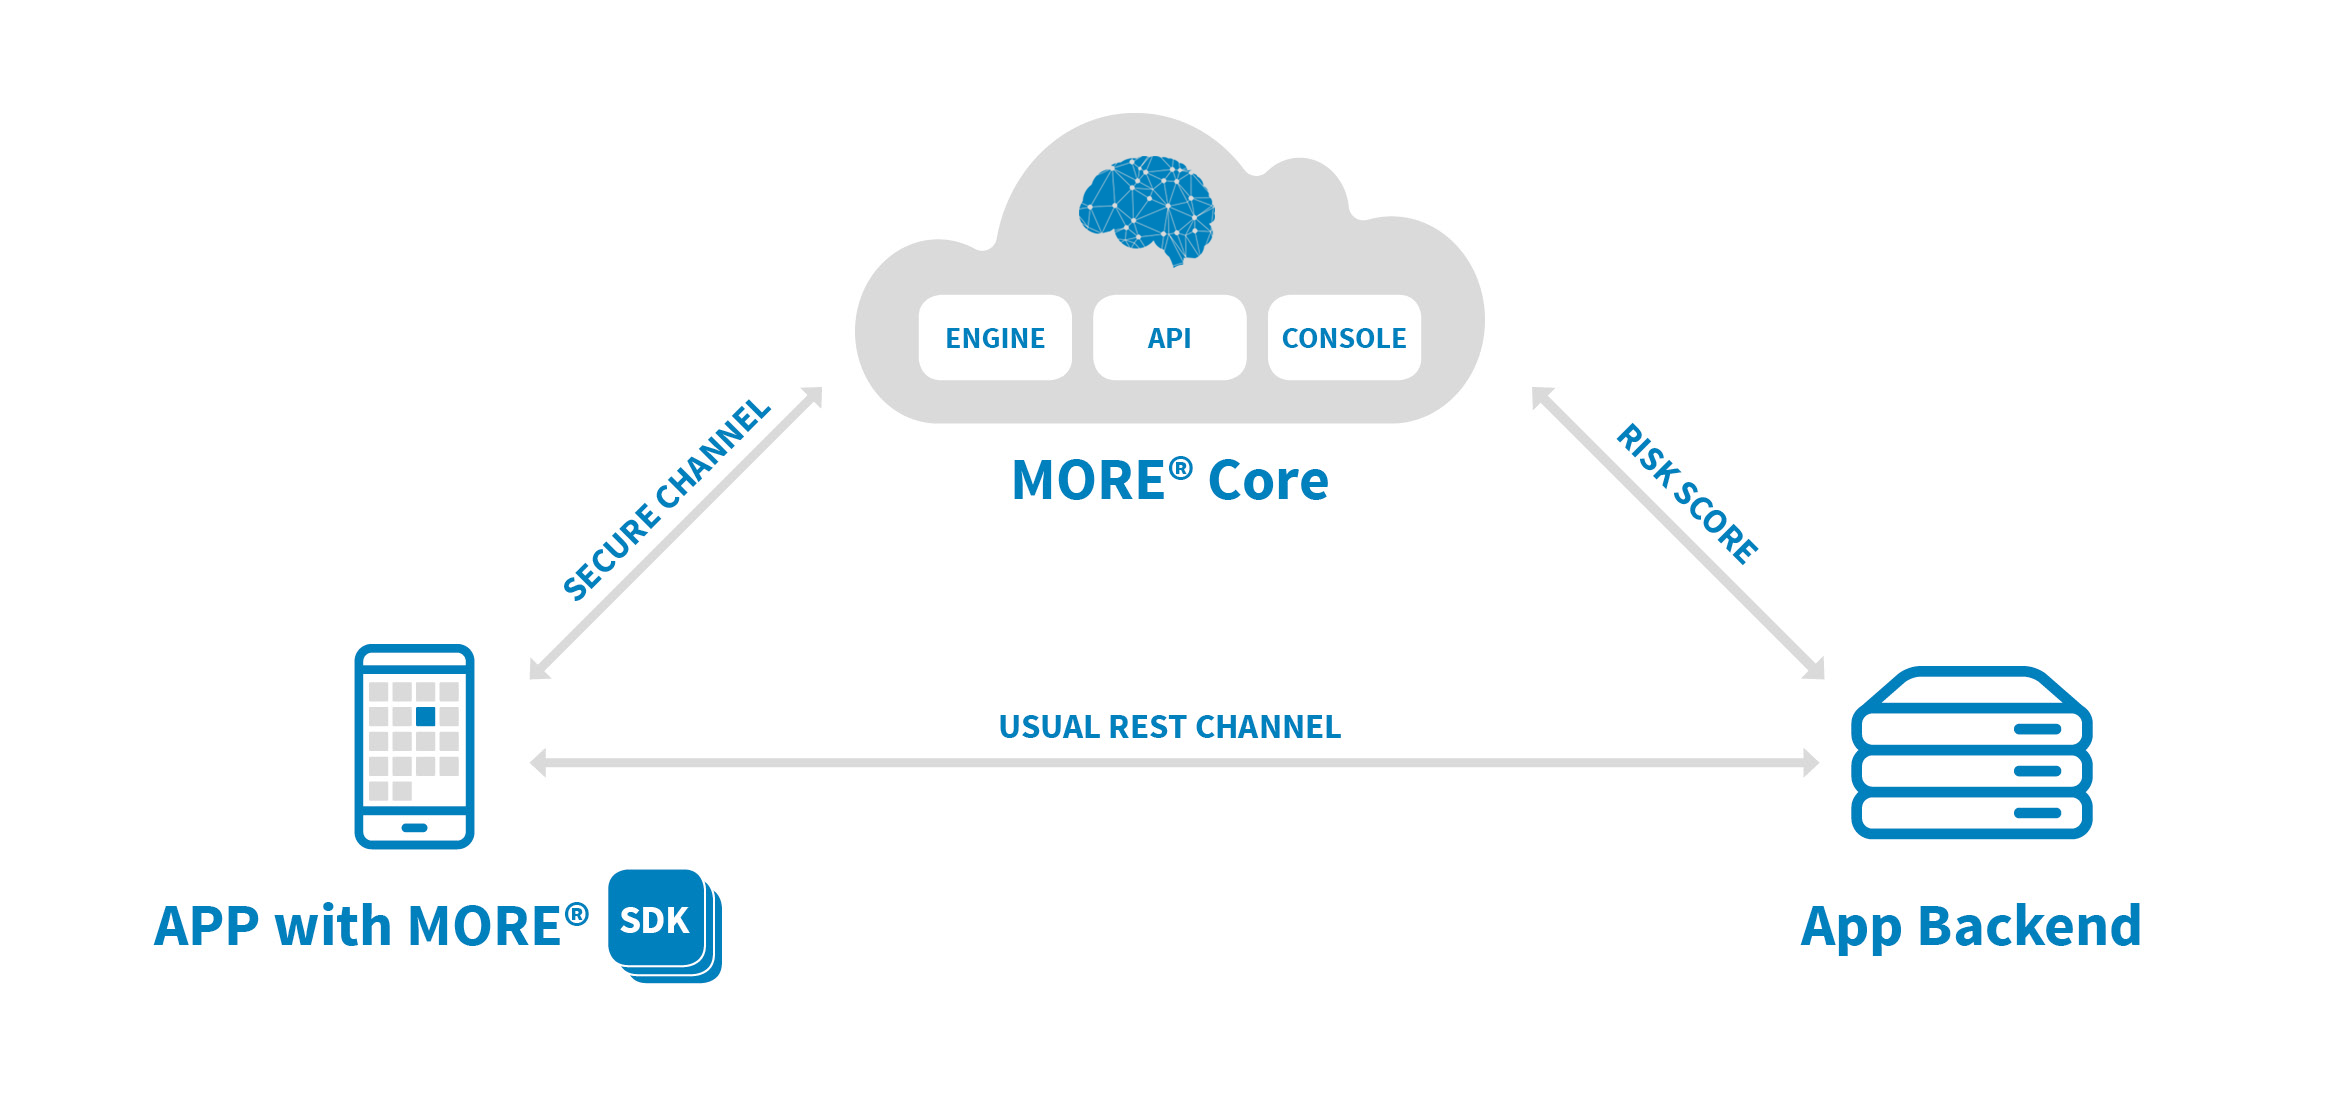
\includegraphics[scale=0.15]{immagini/more-arc.png}
	\caption{\textit{Architettura cloud More\textregistered} (\link{https://xtn-lab.com/more/})}
\end{figure}
\newpage
\section{Organizzazione aziendale}
XTN adotta l'\textit{Agile Team Organisation} tramite \textit{Squads, Chapters, Guilds}.
\begin{figure}[ht]
	\centering
	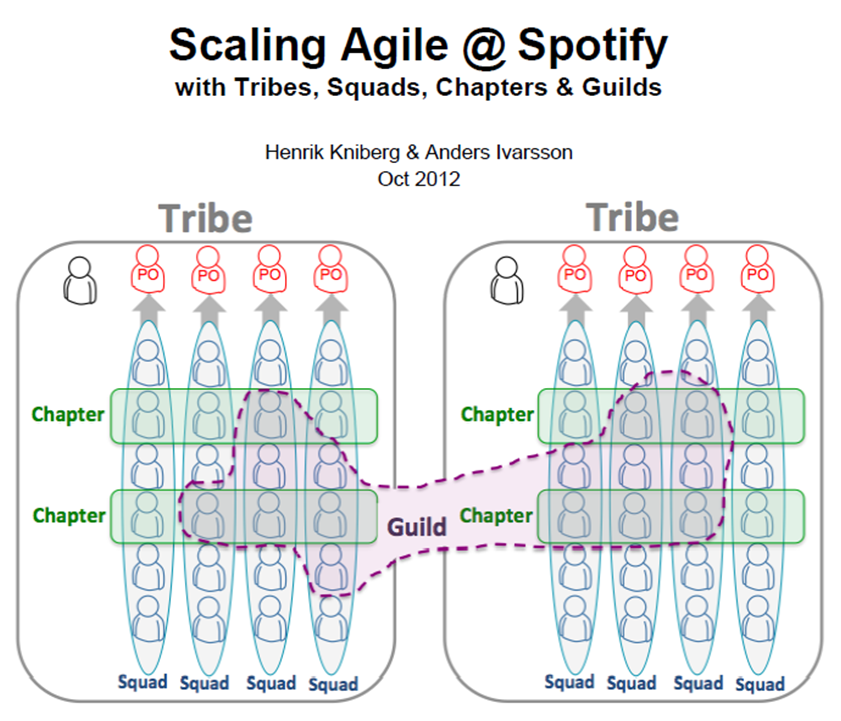
\includegraphics[scale=0.6]{immagini/agile-org.png}
	\caption{\textit{Agile Team Organisation (\link{https://goo.gl/fjJOO6}})}
\end{figure}
\begin{itemize}
\item{\textbf{Squads}:} sono un gruppo di persone che condividono il luogo di lavoro ed il campo di interesse. In XTN esistono due \textit{squads}, uno per  Smash\textregistered\ ed uno per More\textregistered. Ogni \textit{squads} si riunisce periodicamente, circa ogni settimana, per tracciare e discutere la situazione delle varie \textit{milestone}. 
\item{\textbf{Chapters}:} sono un gruppo di persone che condividono le competenze, trasversalmente ai vari \textit{squads}, per promuovere l'innovazione e la collaborazione. Periodicamente, circa ogni mese, i vari \textit{chapters} si riuniscono per condividere informazioni di interesse e favorire un allineamento tecnologico tra i vari \textit{squads}.
\item{\textbf{Guilds}:} sono una comunità di membri, in tutta l'organizzazione, che vogliono condividere conoscenze, strumenti e pratiche comuni. Ad esempio, in XTN, esiste una \textit{guild} nata per accrescere la conoscenza sull'intelligenza artificiale.
\item{\textbf{Tribe}:} sono nate per suddividere, e rendere più gestibile, una grande infrastruttura. XTN non ha adottato questo concetto essendo ancora un azienda di piccole dimensioni.
\end{itemize}
In particolare, durante il periodo di stage, sono stato localizzato nello \textit{squads} di Smash\textregistered\, ma non appartenevo a nessuna \textit{guilds}.
\newpage

\section{Processi aziendali e strumenti di supporto}
In questa sezione verranno affrontati i processi aziendali e le tecnologie a supporto che ho avuto modo conoscere ed imparare lavorando a stretto contatto con il \textit{team} di Smash\textregistered.

\subsection{Gestione della configurazione}
Tutti gli oggetti, che siano documentali e non, sono mantenuti in un \textit{repository} interno. La configurazione è un insieme di questi oggetti che andranno a comporre una determinata versione del prodotto. Ogni configurazione ha il proprio identificativo univoco e un documento contenente informazioni utili all'installazione del prodotto.\\
Ogni oggetto per essere aggiunto ad una determinata configurazione deve essere prima verificato dall'amministratore di progetto.
\subsubsection{Strumenti di supporto}
Per tener traccia di tutte le modifiche ed evitare sovrascritture involontarie l'azienda ha deciso di adottare una repository interna chiamata \textbf{Stash} \footnote{Stash: url= \link{https://it.atlassian.com/}}. Quest'ultima è un sistema di gestione di \textit{repository} che utilizza diversi sistemi di controllo di versione, tra cui Git e Mercurial. Infine l'azienda ha deciso di utilizzare \textbf{Git} \footnote{Git: url= \link{https://git-scm.com/}} come controllo di versione.
\subsection{Processo di sviluppo}
L'azienda si ritrova spesso a dover vendere il proprio prodotto con un certo numero di personalizzazioni. Per far ciò gli addetti alla vendita di XTN effettuano incontri con i clienti per ricavare idee ed osservazioni per, successivamente, stilarli in un documento. Questo documento poi verrà usato dal team di sviluppo per creare il prodotto in linea con le richieste del cliente.\\
L'azienda non rilascia protipi incompleti al cliente ma solamente prodotti funzionanti con tutte le personalizzazioni richieste.\\
Attualmente per ogni personalizzazione richiesta dal cliente il team di sviluppo cerca di renderla una \textit{feauture} usabile da tutti e quindi rivendibile.
\subsubsection{Strumenti di supporto}
\begin{itemize}
\item{\textbf{Backend}}\\
Per quanto riguarda la parte logica l'azienda ha deciso di utilizzare principalmente \textbf{Java} \footnote{Java: url= \link{https://www.java.com/it/}} come linguaggio, in quanto è molto performante ed ha una sintassi molto regolare. Per quest'ultimo il team di sviluppo ha deciso di adottare il \textbf{\gls{framework} Spring} \footnote{Spring: url= \link{https://spring.io/}} per astrarre, e semplificare, buona parte di architettura di \textit{backend}.\\
Per quanto riguarda la persistenza dei dati, XTN, ha deciso di adottare \textbf{MongoDB} \footnote{MongoDB: url= \link{https://www.mongodb.com/it}}.
\begin{figure}[ht]
	\centering
	
\includegraphics[scale=0.15]{immagini/java-spring.png}
	\caption{\textit{Logo Java e Spring (\link{https://goo.gl/Gm7usK})}}
\end{figure}
\newpage
\item{\textbf{Frontend}}\\
Per quanto riguarda l'interfaccia grafica della \textit{dashboard} di Smash\textregistered, XTN ha deciso di adottare il \textbf{\gls{framework} AngularJS 1}\footnote{Angular 1: url= \link{https://angularjs.org/}}. Quest'ultimo è sviluppato da Google e permette di semplificare lo sviluppo e \textit{test} di applicazioni web \textit{single page}.
\begin{figure}[ht]
	\centering
	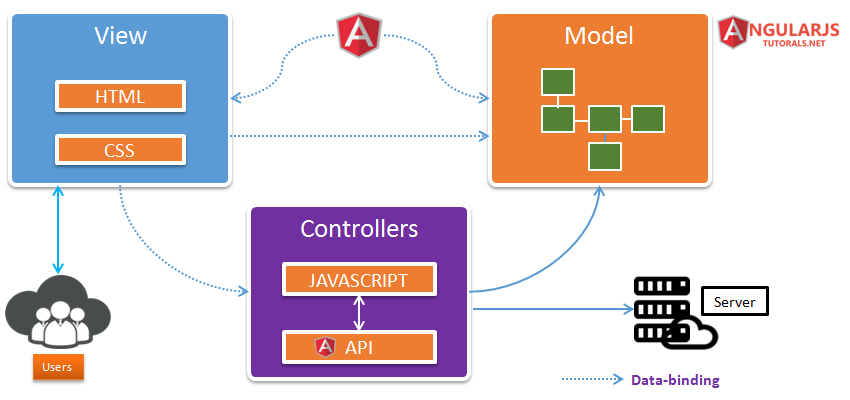
\includegraphics[scale=0.3]{immagini/angular.png}
	\caption{\textit{Architettura AngularJS (\link{https://goo.gl/PzB2v8})}}
\end{figure}
\end{itemize}

\subsection{Processo di manutenzione}
Ogni malfunzionamento viene segnalato e tracciato con la rispettiva priorità. Il personale addetto risolverà le varie segnalazioni in ordine di priorità e successivamente, dopo la sistemazione di un certo numero di malfunzionamenti, il \textit{project manager} rilascerà la nuova versione del prodotto.
\subsubsection{Strumenti di supporto}
Qualunque malfunzionamento viene segnalato e registrato in un sistema di tracciamento delle \textit{issues} chiamato \textbf{Jira} \footnote{Jira: url= \link{https://www.atlassian.com/software/jira}}. Questo servizio permette di assegnare, per ogni \textit{issues}, una priorità, una scadenza e la versione con cui il malfunzionamento sarà sistemato. 
\subsection{Processo di verifica}
Il processo viene gestito dal \textit{chapter} che garantisce la qualità del prodotto offerto. Questo gruppo di persone esegue delle prove per garantire degli \textit{standard}, in ambito di usabilità e prestazioni. Una volta verificate le varie parti il prodotto potrà essere messo in produzione






\section{Rapporto con l'innovazione}
Attualmente i prodotti di \textit{\azienda} hanno raggiunto una maturità tale per cui il servizio che si promettono di offrire coincide con quello che offre realmente. L'azienda, però, continua periodicamete ad investire risorse per trovare nuove tecnologie o soluzioni al fine di offrire un servizio sempre migliore.\\
Queste risorse vengono divise tra studi di settore per focalizzarsi sulle tecnologie del momento e, successivamente, vengono svolti progetti interni, come stage universitari, per verificare la fattibilità della soluzione in analisi. \\
Proprio a questo riguardo, da circa un anno, è in corso uno studio nella tecnologia di \textbf{apprendimento automatico} attraverso corsi di formazione e convegni. Questo viene svolto per riuscire ad aggiungere funzionalità che permettono l'apprendimento automatico del comportamento abituale di determinati utenti. Aggiungere questa funzionalità permetterebbe di abbassare nettamente i falsi positivi di frode bancarie.



% !TEX encoding = UTF-8
% !TEX TS-program = pdflatex
% !TEX root = ../tesi.tex

%**************************************************************
\chapter{Stage come tecnica aziendale}
\label{cap:tecnica-stage}
%**************************************************************

%**************************************************************
\section{Descrizione del progetto}
\textit{\azienda} è il primo anno che attiva progetti di stage in collaborazione con l'Università di Padova. Questo, però, non ha portato a ritardi o disagi per la mancata esperienza, da parte dell'azienda, in questo ambito. 
\subsection{Problema da risolvere per l'azienda}
Tra le tante operazioni che Smash\textregistered\ esegue, esso calcola anche la \textbf{reputazione} che un determinato utente ha.\\
Questa reputazione si suddivide nei 2 seguendi tipi:
\begin{itemize}
\item{\textbf{Reputazione totale}:} è il numero di transazioni bancarie che un determinato utente ha ricevuto.
\item{\textbf{Reputazione relativa}:} è il numero di transazione che un determinato utente ha ricevuto da un utente a scelta.
\end{itemize}
Il fattore di rischio, che Smash\textregistered\ calcola per ogni transazione, è dato anche dalla combinazione di questi 2 tipi di reputazione.\\
Fintanto che la reputazione viene calcolata su un'entità che riceve un numero modesto di transazioni giornaliere la velocità di esecuzione avviene in un tempo accettabile. 
\\Il problema emerge quando questo calcolo viene eseguito su un entità con un enorme numero di transazioni, come può essere un azienda di dominio pubblico che riceve giornalmente transazioni. Questo avviene perchè Smash\textregistered\, per calcolare la reputazione, deve caricare totalmente nella memoria il documento contenente tutte le transazioni di quella determinata azienda.
\subsection{Possibile soluzione}
Il problema potrebbe risolversi utilizzando un determinato tipo di base di dati organizata a \textbf{grafo}.\\
Un grafo è un insieme di \textbf{nodi} che possono essere collegati tra loro attraverso delle relazioni chiamate \textbf{archi}.\\
Questi tipi di base di dati riescono a rappresentare le informazioni utilizzando solamente nodi e archi.
\newpage
\begin{figure}[h!]
	\centering
	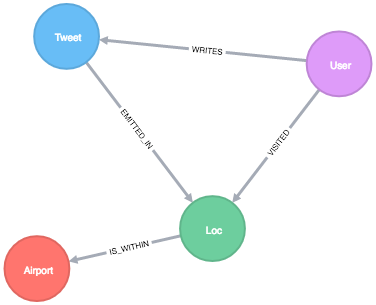
\includegraphics[scale=0.7]{immagini/grafo.png}
	\caption{\textit{Esempio grafo orientato} (\link{https://goo.gl/Z7S8J5)}}
\end{figure}
Un \textbf{nodo} può rappresentare un entità fisica come ad esempio una persona o, in questo preciso contesto, un utente di una banca. Al contrario un \textbf{arco} rappresenta una relazione che avviene tra un nodo ed un altro, come ad esempio una transazione bancaria. Qualsiasi \textbf{nodo} ed \textbf{arco} possono avere un numero a piacere di proprietà, formate da una chiave univoca ed un preciso valore. Inoltre gli \textbf{archi} possono avere un verso di relazione ed un valore che rappresenta il tipo di relazione che l'arco descrive.\\
\textbf{Se l'operazione che calcola la reputazione usasse una rappresentazione dei dati sfruttando la natura dei grafi, il calcolo della reputazione banalmente potrebbe ridursi a contare gli archi entranti di un determinato nodo.} Questo calcolo potrebbe non dipendere dal numero di transazioni che una determinata entità ha ricevuto.\\
Nella figura \hyperref[fig:figura 2.2]{2.2} \textit{Luca} avrebbe una reputazione totale pari a 3 ed una reputazione relativa, rispetto a \textit{Giovanni}, pari a 2.
\begin{figure}[h!]
	\centering
	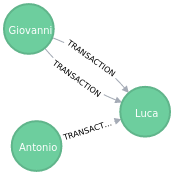
\includegraphics[scale=0.8]{immagini/grafo1.png}
	\label{fig:figura 2.2}
	\caption{\textit{Possibile implementazione della base di dati}}
\end{figure}
\subsection{Direttive del progetto di stage}
Il mio tutor aziendale, \textit{Giuseppe Pavan}, mi ha incaricato di svolgere un'analisi sulle principali tecnologie che adottano una base di dati a grafo e , successivamente, sviluppare un prototipo che cercasse di risolvere il problema precedentemente descritto.\\
L'unico vingolo imposto dal mio tutor aziendale è l'utilizzo del linguaggio Java, visto l'uso massiccio che ne fa Smash\textregistered.\\
Gli obiettivi sono stati suddivisi dal mio tutor aziendale in due categorie: obbligatori e facoltativi.\\
\\
Gli \textbf{obiettivi obbligatori} sono:
\begin{itemize}
\item{\textbf{Documentazione}:} sviluppare un documento contenente la descrizione dettagliata del lavoro di valutazione e identificazione delle soluzioni disponibili in ambito delle base di dati a grafo. Il documento descriverà i vari \textit{software} valutati, caratteristiche, vincoli e i razionali rispetto le scelte affrontate.
\item{\textbf{Ambiente Docker\glsfirstoccur}:} predisposizione di un ambiente di lavoro, con le tecnologie scelte, tramite \textit{container Docker}.
\item{\textbf{Sviluppo prototipo}:} sviluppo di una applicazione prototipale in Java che esemplifichi, partendo da un \textit{dataset} di esempio, le capacità relazionali e prestazionali delle tecnologie scelte.
\end{itemize}

Gli \textbf{obiettivi facoltativi} sono:
\begin{itemize}
\item{\textbf{Estensione del dataset}:} aggiungere maggiore complessità nel \textit{dataset} d'esempio.
\item{\textbf{Presentazione}:} preparazione di una presentazione interna da esporre al \textit{team} focalizzato sull'ambito anti frode.
\end{itemize}
\newpage
\subsection{Pianificazione}
\label{sec:pian}
La pianificazione del progetto di stage l'ha eseguita il mio tutor aziendale nel seguente modo:

\label{tab:pian}
\begin{table}[!ht]

\begin{tabularx}{\textwidth}{lXl}
\hline\hline
\textbf{Giorni} & \textbf{Attività} \\
\hline
3	& Introduzione ad ambito anti-frode focalizzato su transazioni di pagamento (descrizione degli scenari d'uso, delle tipologie di transazioni, attori coinvolti, aspetti di sicurezza e scenari di attacco)\\
\hline
2	& Definizione del problema di correlazione delle transazioni di pagamento e definizione dei requisiti\\
\hline
9	& Analisi dello stato dell'arte relativo alla tecnologia di dase di dati a grafo: identificazione delle diverse tecnologie disponibili, analisi degli elementi differenti, analisi dei requisiti e documentazione\\
\hline
5	& Progettazione del prototipo dimostrativo sfruttando soluzione proposta\\
\hline
15	& Implementazione della soluzione\\
\hline
3	& Validazione e test \\
\hline
2	 & Documentazione\\
\hline
1	& Presentazione interna dell'attività svolta\\
\hline
\end{tabularx}
\\
\caption{Tabella della pianificazione del progetto di stage}
\end{table}%



\begin{figure}[h!]
	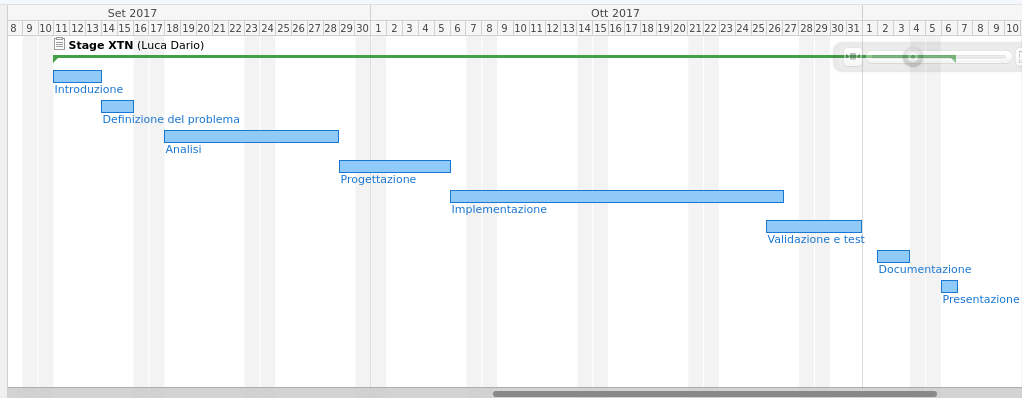
\includegraphics[scale=0.4]{immagini/gant.png}
	\caption{\textit{Diagramma di Gantt della pianificazione del progetto di stage}}
\end{figure}
La pianificazione descritta nella \hyperref[tab:pian]{tabella 2.1} soddisfa, quindi, i vincoli di durata attestandosi sui 40 giorni lavorativi corrispondenti a 320 ore.\\
\subsection{Metodologia e interazione con il tutor aziendale}
Ho deciso, in comune accordo con il tutor aziendale, che l'attività di stage dovesse essere svolta in loco presso la sede di Padova. Questo, oltre a favorire il dialogo con il tutor interno, da l'opportunità di confrontarsi assieme ad un personale con esperienza decennale nel campo dello sviluppo ed anti frode.
\newpage

\section{Aspettative aziendali}
Grazie al progetto di stage l'azienda spera di ricevere un'accurata analisi ed una possibile soluzione al problema affrontato precentemente. Questo servirà in futuro come inizio di un \textbf{analisi di fattibilità} per verificare la possibilità di adottare le tecnologie affrontate anche nei loro prodotti. Un'analisi di questo genere in un azienda rischierebbe di avere una priorità di esecuzione bassa con il rischio che questa attività non venga mai eseguita. Grazie al progetto di stage questo problema verrebbe soppiantato, insieme ad  un grosso abbattimento dei costi.

\section{Aspettative personali}
I miei obbiettivi iniziali prima della scelta del progetto di stage erano:
\begin{itemize}
\item conoscere nuove tecnologie.
\item entrare a contatto con le dinamiche del mondo del lavoro.
\item poter offrire un contributo concreto ed utile all'azienda che mi ospitava.
\item condurre un buon stage per poter sviluppare una buona tesi.
\end{itemize}
Considerando i miei obiettivi e la lista delle aziende iscritte a \textit{Stage-It}, ho deciso di scegliere questo progetto in particolare per la sua natura. Questo offre un buon compromesso tra ore spese per l'analisi ed ore per la progettazione e sviluppo. Le ore spese nell'analisi, oltre ad un \textbf{arricchimento personale}, mi permettono di scrivere una \textbf{buona tesi}. Invece le ore spese nello sviluppo mi permettono di \textbf{accrescere le mie conoscenze tecniche e di dinamiche aziendali}. \\
Successivamente alla mia scelta i miei obiettivi aumentarono, anche grazie al tema trattato dal progetto, tra cui:
\begin{itemize}
\item Mettersi in gioco per cercare di concludere tutti gli obiettivi del piano di lavoro nel miglior modo possibile. Questo mi permetterebbe di eseguire una buona presentazione del lavoro svolto in azienda.
\item Conoscere le dinamiche di rilevazione di una frode bancaria.
\item Lavorare con persone con esperienza decennale.
\item Sviluppare conoscenze in un ambito nuovo, tra cui base di dati a grafo e \textit{framework avanzati}.
\item Essere d'aiuto per risolvere un problema reale ad un azienda significativa nel loro settore.
\end{itemize}







% !TEX encoding = UTF-8
% !TEX TS-program = pdflatex
% !TEX root = ../tesi.tex

%**************************************************************
\chapter{Resoconto dello stage}
\label{cap:resoconto-stage}
%**************************************************************

%**************************************************************
\section{Pianificazione}
Prima dell'inizio del progetto di stage, insieme al mio tutor aziendale, abbiamo stilato le attività principali che avrei dovuto svolgere durante il periodo a disposizione. Queste attività sono riportate nella \hyperref[tab:pian]{tabella 2.1}.\\
Il mio tutor ha deciso che, successivamente all'attività di analisi, avrei dovuto svolgere un colloquio con lui per decidere insieme le tecnologie più promettenti e valide nel contesto di anti frode.\\
Durante i primi giorni di stage abbiamo anche svolto vari colloqui per pianificare in dettaglio le varie attività, le modalità di scelta in base al loro ambito di sviluppo e le tecnologie consigliate.

\section{Analisi}
\subsection{Introduzione}
Nei primi giorni di stage io ed il mio tutor abbiamo deciso i principali punti su cui analizzare le varie tecnologie. Questi sono conseguenti all'ambito di sviluppo dell'azienda e le tecnologie che già adottano.\\
I punti di interesse solo:
\begin{itemize}
\item{\textbf{Licenza:}} verificare che tipo di licenza ha il prodotto, se ha una versione gratuita e che tipo limitazioni ha rispetto a quella a pagamento.
\item{\textbf{Tipo:}} verificare il tipo di tecnologia implementata, se una base di dati a \gls{grafo nativa}o \gls{non nativa}.
\item{\textbf{Modelli disponibili:}} verificare che tipi di \gls{modelli} offre.
\item{\textbf{Community:}} verificare l'ampiezza della \textit{community} del prodotto in analisi, avendola molto sviluppata é possibile ricercare consigli o risoluzioni di determinati problemi nei vari \textit{forum} di riferimento.
\item{\textbf{Tecnologie sopportate nativamente (di rilievo per l'azienda):}} verificare se la tecnologia mette a disposizione un supporto a tecnologie di riferimento all'azienda quali Java o Spring.
\item{\textbf{Linguaggio di interrogazione proprietario:}} verificare se la tecnologia in analisi mette a disposizione un linguaggio di interrogazione proprietario e ottimizzato per essa, analizzando la sua espressività.
\item{\textbf{Supporto Tinkerpop\footnote{Tinkerpop: url= \link{http://tinkerpop.apache.org/}}:}} verificare se la tecnologia mette a disposizione il supporto ad Apache Tinkerpop, sfruttando quindi un interfaccia comune, permettendo poi il passaggio ad un altra tecnologia che lo supporti a costi nulli.
\item{\textbf{\gls{Clustering}:}} verificare se la tecnologia mette a disposizione un sistema di \textit{clustering} pronto all'uso, il tipo e se ha la possibilitá di eseguire \textit{query} distribuite. Infine verificare se questa é disponibile nelle versione gratuita.
\item{\textbf{Security:}} verificare che sistemi di sicurezza dei dati la tecnologia mette a disposizione e se esiste la possibilità di dividere il \textit{database} in zone facendole diventare accessibili solo a determinati utenti.\\

\end{itemize}
Le informazioni necessarie all'analisi le ho reperite in primo luogo dalle documentazioni ufficiali delle case produttrici e successivamente dai \textit{forum} quali StackOverflow\footnote{StackOverflow: url= \link{https://stackoverflow.com/}} e Dzone\footnote{Dzone: url= \link{https://dzone.com/}}.
\subsection{Tecnologie in analisi}
Le tecnologie le ho scelte in base a quelle più diffuse o più promettenti sulla carta attraverso ricerche su internet.
\begin{figure}[h!]
	\centering
	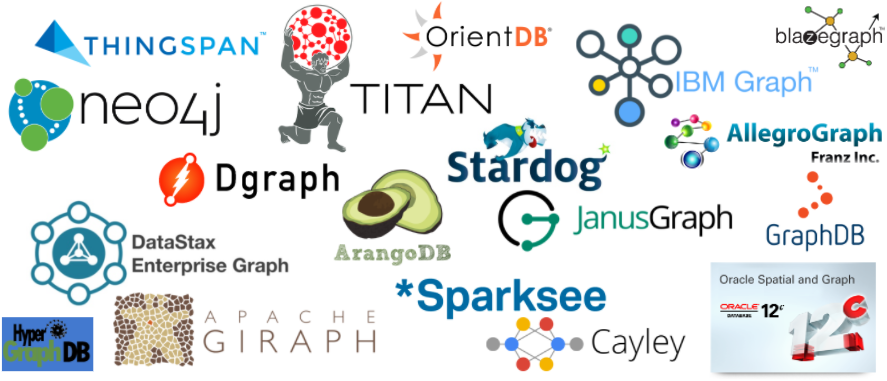
\includegraphics[scale=0.35]{immagini/graphdb.png}

	\caption{\textit{Alternative tecnologiche nel mercato \link{https://goo.gl/d3UUgT}}}
\end{figure}

\subsubsection{Sparksee(DEX)}
Sparksee\footnote{Sparksee: url= \link{http://www.sparsity-technologies.com/}} è un grafo nativo sviluppato in C++ da Spark Technologies a fine 2008 sotto nome DEX. Successivamente nel 2014 cambia nome in Sparksee.\\
È stato il primo \textit{database} a grafo disponibile per Android e iOS.\\
Supporta tecnologie di rilievo per l'azienda come Java, Maven e viene rilasciato per Linux, MacOs, Windows e per i principali sistemi operativi mobili.
La casa produttrice dichiara come caso d'uso possibile il rilevamento di frode bancarie.\\
Questa tecnologia viene rilasciata solamente in versione con licenza commerciale ed accademica con il limite ad un milione di nodi.

\subsubsection{Neo4j}
Neo4j\footnote{Neo4j: url= \link{https://neo4j.com/}} è la base di dati a \gls{grafo nativa} più diffusa al mondo, e, anche grazie a questo, ha una \textit{community} molto ampia. È un \textit{software} sviluppato in Java da Neo Technology nel 2007. È adottato da multinazionali come Microsoft, AirBnb, IBM, Ebay.\\
Neo4j ha un linguaggio di interrogazione proprietario, chiamato Chyper, molto espressivo e ottimizzato. Supporta le tecnologie di rilievo per l'azienda, compreso Spring Data\footnote{Spring data: url= \link{http://projects.spring.io/spring-data/}}. Neo4j viene rilasciato in versione \textit{community} gratuita con nessuna limitazione di ampiezza della base di dati senza la possibilità di eseguirlo in modo distribuito, al contrario di quella \textit{Enterprise} a pagamento.

\subsubsection{ArangoDB}
ArangoDB\footnote{ArangoDB: url= \link{https://www.arangodb.com/}} è un \textit{database} multi modello sviluppato in C++ nato nel 2011. È un \textit{database} principalmente documentale ma con collezioni che, raccogliendo la chiave di entrata e di uscita, simulano il funzionamento a grafo. Questo permette di organizzare i dati utilizzando il modello a grafo, documentale e chiave/valore.\\
Gli sviluppatori promettono la flessibilità data dalle base di dati multi modello e velocità paragonabile ai \textit{database} a grafo nativi.\\
ArangoDB ha un linguaggio di interrogazione proprietario simile ad \gls{SQL} e viene rilasciato in versione gratuita con limitazioni solo nell'ambito della sicurezza.
\subsubsection{AllegroGraph}
AllegroGraph\footnote{AllegroGraph: url= \link{https://franz.com/agraph/allegrograph/}} è un software per \textit{database} a grafo nativo sviluppato insieme agli \textit{standard} W3C\footnote{W3C: url= \link{https://www.w3.org/}} per il \textit{web} \gls{semantico}  nel 2004. Supporta tecnologie di interesse all'azienda ma non ha un linguaggio di interrogazione proprietario. Viene rilasciato solo con licenza commerciale a pagamento.
\subsubsection{OrientDB}
OrientDB\footnote{OrientDB: url= \link{http://orientdb.com/orientdb/}} è un \textit{software} per base di dati multi modello sviluppato in Java da uno sviluppatore italiano chiamato Luca Garulli\footnote{Luca Garulli: url= \link{https://www.linkedin.com/in/garulli}}. È un \textit{database} principalmente documentale ma, salvando attraverso tabelle gli indici fisici di inizio e fine dell'arco, riesce ad implementare anche il modello a grafo nativo. \\
Per scelta puramente commerciale hanno deciso di integrare un linguaggio di interrogazione molto simile a \gls{SQL}, limitando di molto l'espressività nelle ricerche nel modello a grafo. Viene rilasciato in versione sia a pagamento che \textit{community} con nessuna limitazione di rilievo.
\subsubsection{Titan}
Titan\footnote{Titan: url= \link{http://titan.thinkaurelius.com/}} è un software in grado di sfruttare \textit{storage backend} come Apache Cassandra\footnote{Apache Cassandra: url= \link{http://cassandra.apache.org/}} per l'immagazzinamento dei dati. È capace di astrarre i dati nello \textit{storage} ed organizzarli come se fossero a grafo, di conseguenza non utilizza una base di dati a \gls{grafo nativa}.
Questa possibilità di scelta dello \textit{storage backend} lo rende molto valido se l'azienda utilizzasse una tecnologia che lo supporta, questo porterebbe ad un costo di passaggio tecnologico più contenuto.\\
Titan non offre un linguaggio di interrogazione proprietario ma supporta pienamento Tinkerpop.  Viene rilasciato in licenza Apache 2\footnote{Apache 2: url= \link{https://www.apache.org/licenses/LICENSE-2.0}}.
\subsection{Scelta tecnologica}
\begin{figure}[h!]
	\centering
	
\includegraphics[scale=0.45]{immagini/neo4j.png}
	
\includegraphics[scale=0.3]{immagini/orientdb.png}
	\caption{\textit{Logo \href{https://neo4j.com/}{Neo4j} e \href{http://orientdb.com/orientdb/}{OrientDB}}}
\end{figure}
Dopo un colloquio dove ho mostrato al mio tutor i risultati dell'analisi, in comune accordo abbiamo scelto le due tecnologie più promettenti ed interessanti.\\
Abbiamo scelto \textbf{Neo4j} per il suo linguaggio di interrogazione molto espressivo e la sua diffusione a livello mondiale che porta ad una \textit{community} molto attiva.\\
Infine abbiamo scelto anche \textbf{OrientDB} essendo il \textit{database} multi modello più promettente sulla carta che organizza i dati come uno a grafo nativo.
\\
\\

\section{Sviluppo del prototipo}
\subsection{Analisi dei requisiti}
La prima attività svolta, dopo l'analisi delle tecnologie, è stata l'analisi dei requisiti. Questo perché l'organizzazione della base di dati deve essere strutturata in modo tale da semplificare le operazione che il prototipo andrà ad eseguire.\\
Ho tracciato tutti i requisiti utilizzando il seguente schema.\\
\begin{itemize}
	\item \textbf{Importanza:} può assumere questi valori:
  		\begin{itemize}
    		\item \textbf{1:} indica un requisito obbligatorio;
    		\item \textbf{2:} indica un requisito opzionale;
  		\end{itemize}
  	\item \textbf{Tipo:} può assumere questi valori:
  		\begin{itemize}
   		 	\item \textbf{F:} indica un requisito funzionale;
    		\item \textbf{Q:} indica un requisito di qualità;
    		\item \textbf{V:} indica un requisito di vincolo.
  		\end{itemize}
  	\item \textbf{Identificativo:} indica il codice identificativo del requisito, è un intero positivo crescente.
\end{itemize}
Ho definito tutti i requisiti tramite \textit{brainstorming} con il mio tutor aziendale e definiti nella seguente tabella.
\label{tab:rec}
\begin{table}[!ht]
\begin{tabularx}{\textwidth}{Xll}
\hline\hline
\textbf{Requisito} & \textbf{Identificativo} \\
\hline
Stesura documento con descrizione dettagliata dell'analisi svolta. & 1V1\\
\hline
Predisposizione di un ambiente di lavoro con il \textit{database} scelto utilizzando \textit{deploy} tramite container docker. & 1V2\\
\hline
Sviluppo prototipo & 1V3\\
\hline
Preparazione ed esecuzione di una presentazione. & 2V4\\
\hline
Estensione del \textit{dataset} considerato e aggiunta di maggiore complessità nelle relazioni valutate. & 2V5\\
\hline
Il prototipo deve permettere il calcolo della reputazione totale & 1F6\\
\hline
Il prototipo deve permettere il calcolo della reputazione relativa & 1F7\\
\hline
Il prototipo deve permettere l'aggiunta di una transazione & 1F8\\
\hline
Il prototipo deve permettere l'aggiunta di un \textit{AccountId} & 1F9\\
\hline
Il prototipo deve permettere l'aggiunta di un \textit{EntityId} & 1F10\\
\hline
Il prototipo deve permettere di associare un \textit{AccountId} ad un \textit{EntityId} & 1F11\\
\hline
Il prototipo deve permettere l'eliminazione di un \textit{AccountId} & 1F12\\
\hline
Il prototipo deve permettere l'eliminazione di un \textit{EntityId} & 1F13\\
\hline
La copertura dei test di unità deve essere maggiore o uguale al 85\% & 1Q14\\
\hline
Il prototipo deve permettere il calcolo dell'ammontare delle transazioni da una certa data in poi rispetto un \textit{AccountId} & 2F15\\
\hline
Il prototipo deve riuscire a calcolare la somma delle reputazioni totali di tutti gli \textit{AccountId} associati ad un \textit{EntityId} & 2F16\\
\hline
Il prototipo deve riuscire a calcolare la somma delle reputazioni relative di tutti gli \textit{AccountId} associati ad un \textit{EntityId} & 2F17\\
\hline
Soddisfacimento del 100\% dei requisiti obbligatori & 1F18\\
\hline
\end{tabularx}
\caption{Tabella tracciamento requisiti.}
\end{table}%
\\
Tutti i requisiti descritti sono stati poi approvati dal mio tutor aziendale.
\newpage
\subsection{Tecnologie utilizzate}
Tutte le tecnologie che ho utilizzato sono state accordate preventivamente con il tutor aziendale.
\subsubsection{IntellJ Idea Ultimate}
Ho utilizzato IntellJ Idea, con licenza accademica, come \gls{IDE} in primo luogo per la conoscenza maturata dai progetti passati eseguiti in ambito universitario. Inoltre integra il supporto a JUnit\footnote{JUnit: url= \link{http://junit.org/junit5/}} per facilitare i \textit{test}, a Maven per eseguire la \textit{Build} direttamente dall'\gls{IDE}, \textit{debugger} avanzato. In aggiunta offre anche molte funzionalità utili come la possibilità di eseguire \textit{\gls{refractoring}} con la certezza che il comportamente resti invariato.

\subsubsection{Java 8}
Ho utilizzato Java come linguaggio di programmazione perché, in primo luogo, era un vincolo dettato dal piano di lavoro descritto nella \hyperlink{sec:pianodl}{sezione 2.1.3}. Inoltre questo linguaggio ha una sintassi molto regolare e semplice. Infine essendo uno dei linguaggi più diffusi al mondo ha una vasta quantità di librerie supportate.
\subsubsection{Maven}
Maven\footnote{Maven: url= \link{https://maven.apache.org/}} è uno strumento per la gestione di progetti \textit{software} sviluppato da Apache Software Foundation\footnote{https://www.apache.org/}. Permette di dichiarare tutte le dipendenze e le varie versione delle librerie in un unico file in formato XML\footnote{XML: url\link{https://it.wikipedia.org/wiki/XML}}, separando le \textit{directory} di progetto dalle librerie utilizzate. Maven scaricherà automaticamente le dipendenze e le nasconderà in cartelle separate dal progetto.\\
La \textit{build standard} automatica consiste in diversi passi ordinati e dipendenti l'uno dall'altro tra cui la compilazione, l'esecuzione dei \textit{test}, la verifica. Questo ciclo di \textit{build standard} sarà completato solamente se tutte la varie fasi non genereranno errori.
\begin{figure}[h!]
	\centering
	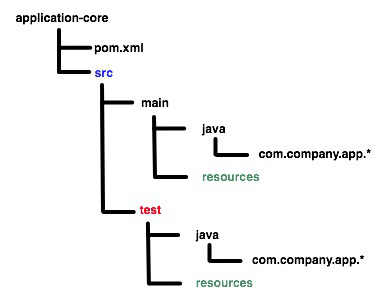
\includegraphics[scale=0.5]{immagini/maven.jpg}
	\caption{\textit{Struttura standard delle cartelle} \link{https://goo.gl/N94Uqs}}
\end{figure}
\subsubsection{Spring Boot}
\begin{figure}[h!]
	\centering
	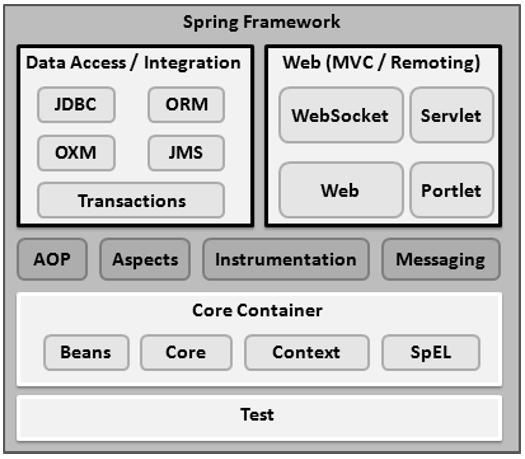
\includegraphics[scale=0.45]{immagini/spring.png}
	\caption{\textit{Architettura del \gls{framework} Spring} \link{https://goo.gl/2hvVYM}}
\end{figure}
Spring Boot\footnote{Spring Boot: url= \link{https://projects.spring.io/spring-boot/}} è un \gls{framework} per semplificare la creazione di progetti Java \textit{stand-alone}. Con questo \gls{framework} è possibile definire l'architettura interna di un progetto, ad esempio un \textit{web server}, con semplici annotazioni Java.\\
Per la creazione di un progetto Spring Boot basta recarsi in \link{https://start.spring.io/}, configurare il nome del progetto e scaricare il sorgente.\\
Spring è una valida alternativa a Enterprise JavaBeans\footnote{Enterprise JavaBeans: url= \link{https://it.wikipedia.org/wiki/Enterprise\textunderscore JavaBeans}}.

\subsubsection{Spring Data Neo4j}

Spring Data Neo4j\footnote{Spring Data Neo4j: url= \link{https://projects.spring.io/spring-data-neo4j/}} è una particolare implementazione di Spring Data\footnote{Spring Data: url= \link{http://projects.spring.io/spring-data/}}. Questa libreria permette di astrarre le operazioni che si eseguono nella base di dati Neo4j semplificando lo sviluppo.\\
Utilizzando questa libreria è possibile definire delle \textit{query} solo grazie alle segnatura dei metodi, questo permette sia velocizzare lo sviluppo sia l'attività di verifica visto che sarebbe inutile eseguirla in un metodo già verificato dalla casa produttrice. Infine permette di eseguire il \textit{map} degli oggetti Java nel \textit{database} semplicemente con delle annotazioni senza generazione di codice.
\begin{figure}[h!]
	\centering
	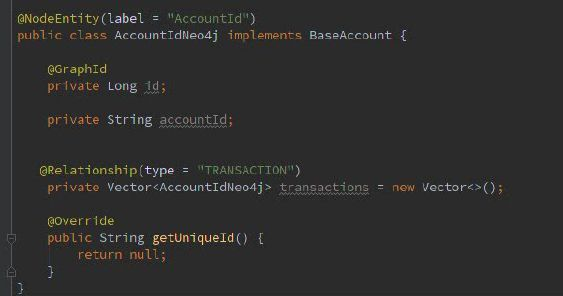
\includegraphics[scale=0.33]{immagini/sdata.jpg}
	\caption{\textit{Esempio di Nodo utilizzando Spring Data Neo4j}}
\end{figure}

\subsubsection{Tinkerpop}

Ho utilizzato Tinkerpop\footnote{Tinkerpop: url= \link{http://tinkerpop.apache.org/}} per interfacciarmi con OrientDB in modo semplice, diminuendo le operazioni eseguite esclusivamente tramite \textit{query}. Questa libreria ha il vantaggio di permettere un passaggio ad un altra tecnologia che lo supporta senza modificare il codice. E stata sviluppata da Apache Software Foundation con lo scopo di uniformare il codice volto a interfacciarsi con la maggior parte dei \textit{database} nel mercato.
\begin{figure}[h!]
	\centering
	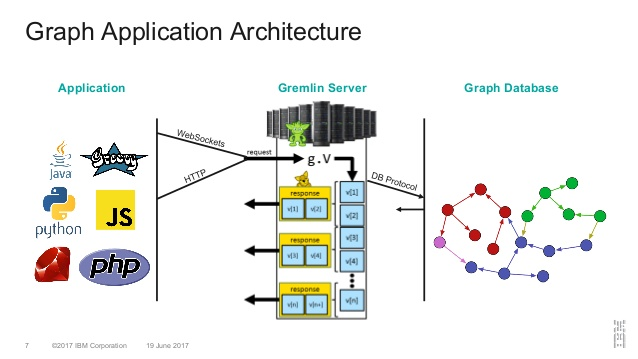
\includegraphics[scale=0.65]{immagini/tinkerpop.jpg}
	\caption{\textit{Architettura di un'applicazione che utilizza Tinkerpop} \link{https://goo.gl/YiXuLB}}
\end{figure}

\subsubsection{JUnit e Mockito}
JUnit\footnote{JUnit: url= \link{http://junit.org/junit5/}} è un \gls{framework} che permette e semplifica la creazione di test in Java. Invece Mockito\footnote{Mockito: url= \link{http://site.mockito.org/}} permette di sovrascrivere il comportamente di un particolare metodo impostandogli i valori di entrata e di uscita. Questo è utile quando si sviluppano i \textit{test} di unità e si utilizzano delle particolari classi non sviluppate o semplicemente non coperte da \textit{test}.
\newpage
\begin{figure}[h!]
	\centering
	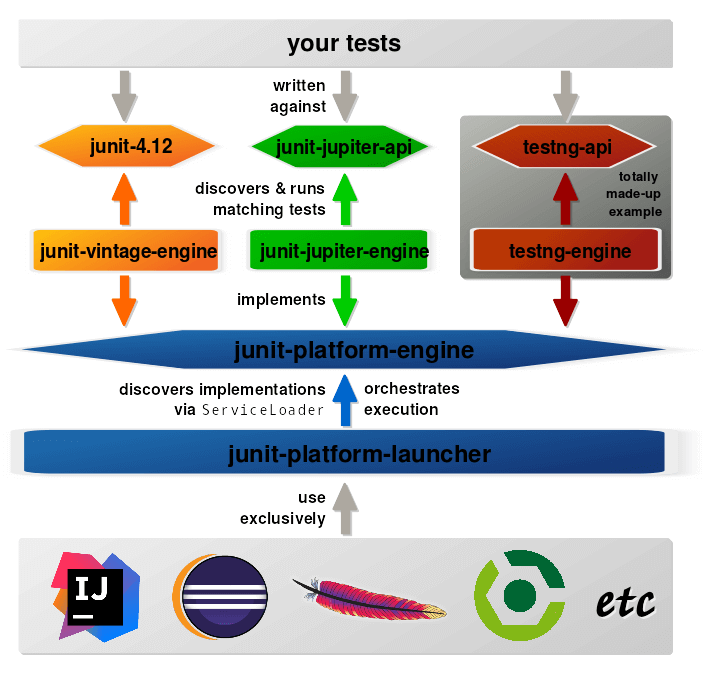
\includegraphics[scale=0.27]{immagini/junit.png}
	
	\caption{\textit{Architettura di JUnit \link{https://goo.gl/6Xgy5U}}}
\end{figure}




\subsection{Base di dati}
In base al problema descritto nella \hyperref[sec:prob]{sezione 2.1.1}, dinamiche di Smash\textregistered\ ed i requisiti descritti nella \hyperref[tab:rec]{tabella 3.1} ho organizzato i dati, per tutti e due i \textit{database}, nel seguente modo:
\begin{itemize}
\item{\textbf{Nodi:}}
\begin{itemize}
\item{\textbf{EntityId:}} è il nodo che rappresenta un utente di una banca, esso può sia svolgere transazioni verso un \textit{AccountId} che avere relazioni di appartenenza verso uno, o più, \textit{AccountId}.
\item{\textbf{AccountId:}} è il nodo che rappresenta una coordinata bancaria ad esempio un iban, esso può avere transazioni verso altri \textit{AccountId} ed avere massimo una relazione di appartenenza da un \textit{EntityId} a questo nodo.
\end{itemize}
\item{\textbf{Archi:}}
\begin{itemize}
\item{\textbf{TRANSACTION:}} è l'arco che rappresenta una transazione, questo può provenire da un \textit{AccountId} o \textit{EntityId} verso un \textit{AccountId}. Questo ha diverse proprietà tra cui di obbligatorie la data di avvenuta transazione, l'importo e la valuta, e di non obbligatorie come la città e il paese dove è stata eseguita la transazione.
\item{\textbf{OWN:}} è l'arco che descrive la relazione di appartenenza da un \textit{EntityId} ad un \textit{AccountId}. Un \textit{EntityId} può avere un numero a piacere di relazioni di appartenenza, al contrario un \textit{AccountId} può avere al massimo un arco entrante di tipo \textit{OWN}.
\end{itemize}
\end{itemize}
\newpage
\begin{figure}[!ht]
	\centering
	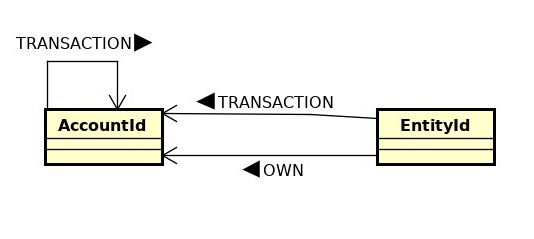
\includegraphics[scale=0.4]{immagini/graph.jpg}
	\caption{\textit{Schema della base di dati}}
\end{figure}
A causa dei problemi legati alle politiche della protezione dei dati sensibili, non ho potuto utilizzare dati reali per il popolamento dei \textit{database} ma ho dovuto creare un progetto per la generarmeli in modo casuale.
\subsection{Prototipo}
\begin{figure}[h!]
	\centering
	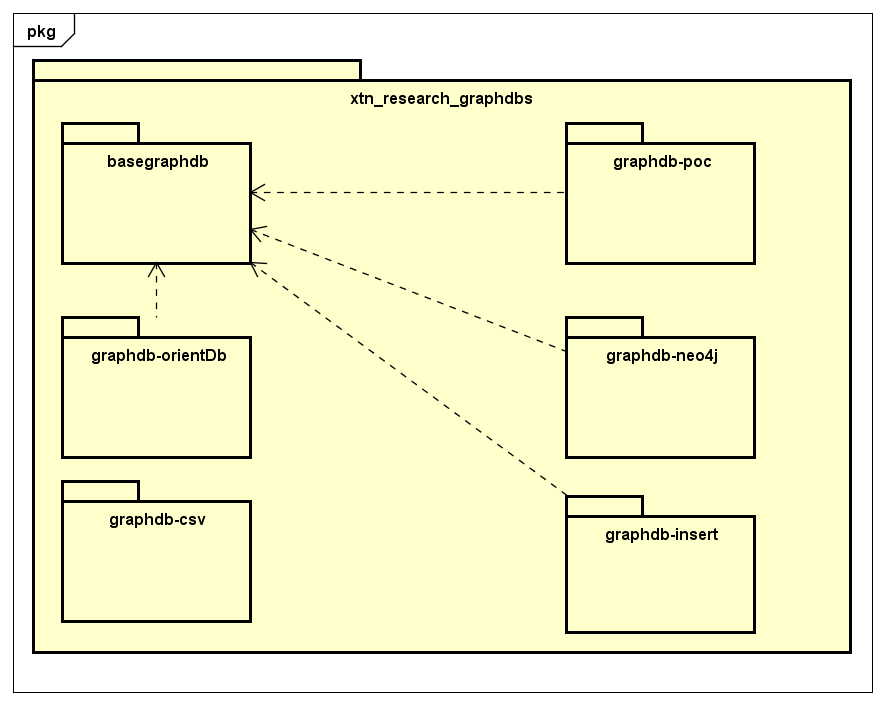
\includegraphics[scale=0.4]{immagini/packages.png}
	\caption{\textit{Diagramma dei package del prototipo}}
\end{figure}
Ho deciso di dividere il prototipo in più progetti sotto l'unico \gls{aggregato Maven} chiamato \textit{xtn\textunderscore research\textunderscore graphdbs}. Questa tecnica l'ho utilizzata per gestire tutte le versioni delle dipendenze in un unico file di configurazione, e, sopratutto, per avere la comodità di eseguire la \textit{build} di tutti i progetti in un unico comando, lasciando a Maven l'onere di risolvere tutte le dipendenze.\\


\subsubsection{basegraphdb}
\textit{Basegraphdb} é il progetto che contiene le varie interfacce comuni tra cui \textit{ReputationController}. Questa é l'interfaccia comune per gestire la reputazione delle varie entitá presenti nei vari \textit{database}. Ogni implementazione, quindi sia \textit{graphdb-neo4j} che \textit{graphdb-orientDb}, conterrà una classe che la implementerà.
\subsubsection{graphdb-orientdb}
\textit{Graphdb-orientDb} é il progetto per la gestione della reputazione tramite OrientDB, esso ha all'interno una classe chiamata \textit{ReputationControllerOrientDb} che implementa \textit{ReputationController}. Questa implementazione usa Tinkerpop\footnote{Tinkerpop: url=\link{http://tinkerpop.apache.org/}} per interfacciarsi con il \textit{database}.
\subsubsection{graphdb-neo4j}
\textit{Graphdb-neo4j} è il progetto per la gestione della reputazione tramite Neo4j, esso ha all'interno una classe chiamata \textit{ReputationControllerNeo4j} che implementa \textit{ReputationController}. Questa implementazione utilizza \textit{Spring Data Neo4j} per interfacciarsi ed eseguire il \textit{map} degli oggetti Java nel \textit{database}.


\subsubsection{graphdb-csv}
\textit{Graphdb-csv} è il progetto per creare tutti i documenti in formato CSV contenenti le entità per popolare i diversi tipi di \textit{database}. Questo crea dati in modo casuale nei migliori dei casi, cioè ogni \textit{AccountId} ha il proprio \textit{EntityId}.\\

\subsubsection{graphdb-insert}
\textit{Graphdb-insert} inserisce in modo del tutto causale un certo numero, definito dall'utente, di \textit{EntityId, AccountId, Transaction} utilizzando l'interfaccia comune \textit{ReputationController}.\\
\textbf{Questo progetto deve essere usato solo per inserire un modesto numero di nodi ed archi} visto che l'aggiunta di ogni \textit{record} ci impiega 500 millisecondi. In caso contrario è consigliato generarsi i CSV delle entità utilizzando il progetto \textit{graphdb-csv} e successivamente importarli nel \textit{database} scelto.
\subsubsection{graphdb-poc}
\textit{Graphdb-poc} è il progetto che si occupa solamente di instanziare le varie implementazioni di \textit{ReputationController} ed eseguire i vari metodi d'interfaccia tracciando, e stampando a video, il nome del metodo, il risultato ottenuto ed il tempo impiegato.\\
Questo progetto non ha dipendenze verso le varie implementazioni ma solamente verso l'interfaccia. Questo è possibile delegando a Spring l'onere di iniettare tutte le classi che implementano l'interfaccia comune. In questo modo si ha un disaccoppiamento tra questo progetto e le varie implementazioni e, sopratutto, se in futuro ci fosse il bisogno di aggiungerne un altra non sarebbe necessario modificare il codice di questo progetto.
\begin{figure}[!ht]
	\centering
	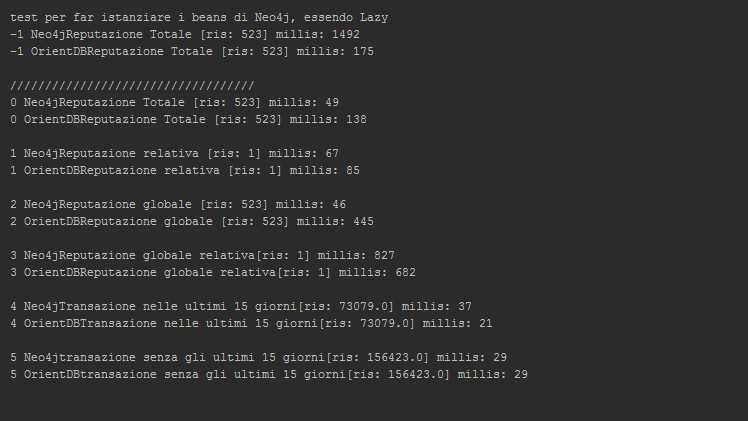
\includegraphics[scale=0.75]{immagini/poc.png}
	\caption{\textit{Risultati stampati da graphdb-poc}}
\end{figure}
\newpage
\section{Utilizzo della libreria}
\subsection{Calcolo della reputazione}
Sfruttando la \textit{dependency injection} \footnote{dependency injection: url= \link{https://en.wikipedia.org/wiki/Dependency\textunderscore injection}} di Spring, per utilizzare la libreria del calcolo della reputazione è sufficiente creare una classe simile alla seguente.
\begin{lstlisting}
package it.ldario;

import it.ldario.graphdbneo4j.ReputationControllerNeo4j;
//import it.ldario.graphdborientDb.ReputationControllerOrientDb;
import org.springframework.beans.factory.annotation.Autowired;
import org.springframework.boot.CommandLineRunner;
import org.springframework.boot.SpringApplication;
import org.springframework.boot.autoconfigure.SpringBootApplication;

@SpringBootApplication
public class MiaClasse implements CommandLineRunner {

    public static void main(String[] args) {
        SpringApplication.run(MiaClasse.class, args);
    }
    
    
	
	//utilizzando, come tipo statico, ReputationControllerNeo4j oppure //ReputationControllerOrientDb verra' usato, rispettivamente //l'implementazione di Neo4j o OrientDB
    private ReputationControllerNeo4j reputationController;
    //private ReputationControllerOrientDb reputationController;



    @Autowired
    public MiaClasse(ReputationControllerNeo4j reputationController) {
        this.reputationController = reputationController;
    }
    

    @Override
    public void run(String... strings) throws Exception {
        //aggiunge al database scelto(orientDB oppure Neo4j), dipende dal tipo //che viene dichiarato, un entity con id="Luca"
        reputationController.addAccountId("Luca");

        //stampa la reputazione totale dell'entity "Luca"
        System.out.println(reputationController.getTotalReputation("Luca"));
        
        

        //stampa il totale delle transazioni effettuate da Luca negli ultimi //15 giorni
		System.out.println(reputationController
        						.getAmountAccountIdInATimeRange("Luca", 15));
        						
        						
        						
        //aggiunge al database scelto(orientDB oppure Neo4j), dipende dal tipo //che viene dichiarato, un account con id "IT123"
        
         TransactionBuilder transactionBuilder = new TransactionBuilder(); 
        transactionBuilder.setCountry("Italy").setCity("San Michele delle Badesse").setAmount(100).setCurrency("Euro");
        reputationController.addTransaction("Luca","IT123",transactionBuilder
        																.build());
        

    }
}
\end{lstlisting}
\subsection{Estensione della libreria con un altro tipo di database}
Per aggiungere un altro tipo di database è necessario solamente creare una classe simile alla seguente, senza modificare il codice del prototipo.
\begin{lstlisting}
package it.ldario.newdatabase;

import it.ldario.basegraphdb.ReputationController;


public class ReputationControllerNewDatabase implements ReputationController {
    //implementazione di tutti i metodi di interfaccia
}
\end{lstlisting}

\subsection{Popolamento della base di dati}
Per aggiungere un numero modesto di dati generati casualmente, in qualunque tecnologia che implementa \textit{ReputationController}, è necessario solamente creare una classe simile alla seguente.
\begin{lstlisting}
package it.ldario;


import it.ldario.graphdbinsert.GraphDbInsertImpl;
import it.ldario.graphdbneo4j.ReputationControllerNeo4j;
//import it.ldario.graphdborientDb.ReputationControllerOrientDb;
import org.springframework.beans.factory.annotation.Autowired;
import org.springframework.boot.CommandLineRunner;
import org.springframework.boot.SpringApplication;


public class MiaClasse implements CommandLineRunner {

    //esplicitando il tipo verra' scelto, rispettivamente, il reputation //controller di Neo4j o OrientDB
    private ReputationControllerNeo4j reputationController;
    //private ReputationControllerOrientDb reputationController;

    public static void main(String[] args) {
        SpringApplication.run(GraphdbPocApplication.class, args);
    }

    @Autowired
    public MiaClasse(ReputationControllerNeo4j reputationController) {
        this.reputationController = reputationController;
    }

    @Override
    public void run(String... strings) throws Exception {
        GraphDbInsertImpl graphDbInsert = new GraphDbInsertImpl(10,20,50,reputationController);

    }
}
\end{lstlisting}
Eseguendo il \textit{Main} si andranno ad aggiungere nel \textit{database} scelto 10 \textit{EntityId}, 20 \textit{AccountId} e 50 Transazioni. Per scegliere la base di dati su cui agire è necessario modificare, con il tipo desiderato, la variabile \textit{reputationController}.




\section{Verifica e validazione}
\subsection{Verifica}
Nell'attività di verifica ho utilizzato JUnit\footnote{JUnit: url= \link{http://junit.org/junit5/}} e Mockito\footnote{Mockito: url= \link{http://site.mockito.org/}} per facilitare la creazione dei \textit{test}.

\begin{figure}[!ht]
	\centering
	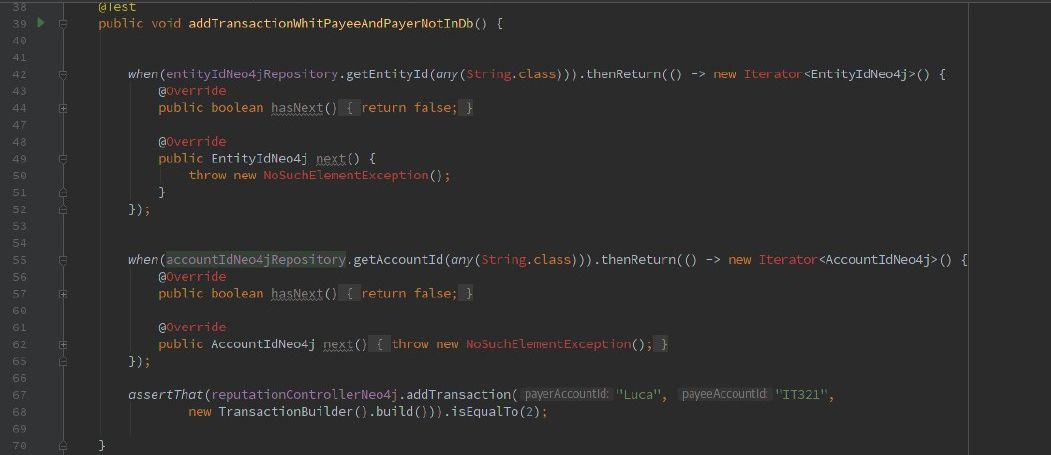
\includegraphics[scale=0.4]{immagini/test.jpg}
	\caption{\textit{Esempio di test utilizzando Mockito e JUnit}}
\end{figure}
Sono state testate tutte le \textit{query} utilizzando un immagine docker\footnote{Docker: url= \link{https://www.docker.com/}} di \textit{test}, escluse quelle banali auto generate da Spring.
Invece per testare le varie unità mi sono aiutato istanziando ed istruendo facilmente dei \textit{mock} utilizzando Mockito.
In accordo con il mio tutor aziendale è stata decisa la soglia minima di copertura dei test del 85\%.\\
La copertura finale dei test si è attestata sul 88\% tra il codice consegnato in azienda.
Ogni test ha uno ed uno solo confronto al suo interno ed ha un nome che indica con precisione che operazioni andrà ad eseguire. Questo ha il vantaggio di sapere esattamente con che condizioni il \textit{test} fallisce solamente leggendo il nome. Inoltre ogni requisito è stato coperto da \textit{test}, questo per verificare l'avvenuto soddisfacimento di esso.\\
Tutti i \textit{test} verificano la logica interna dell'unità e percorrono la quasi totalità dei cammini possibili, questo per far emergere tutti i possibili errori nel codice.
\newpage
\begin{figure}[!ht]
	\centering
	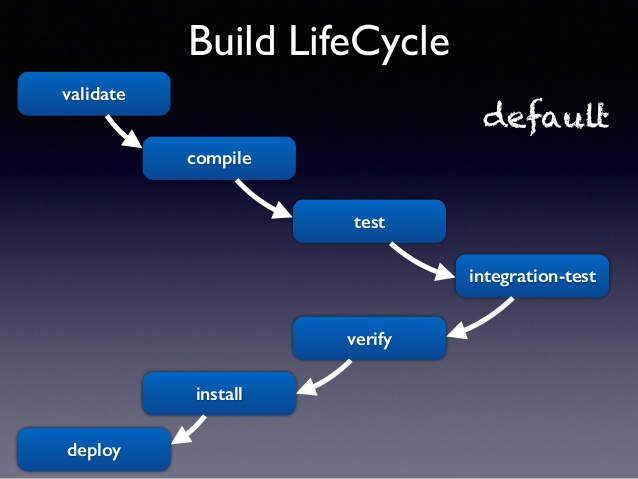
\includegraphics[scale=0.4]{immagini/build.jpg}
	\caption{\textit{Ciclo di vita della build standard di Maven \link{https://goo.gl/gvgZBN}}}
\end{figure}

La \textit{build} non andrà a buon fine se tutti i \textit{test} non avranno esito positivo, questo è gestito completamente e garantito dal processo di \textit{build standard} di Maven.
\subsection{Validazione}
\label{sec:valid}
Per quanto riguarda la validazione ho consegnato un documento, in azienda, contenente tra cui una tabella con il codice del requisito descritto nella \hyperlink{tab:rec}{tabella 3.1} e se è stato soddisfatto.\\
La tabella dei riquisiti obbligatori è la seguente:

\label{tab:pian}
\begin{table}[!ht]
\begin{tabularx}{.35\textwidth}{XX}
\hline\hline
\textbf{Requisito} & \textbf{S\footnote{S: Soddisfatto}/NS\footnote{NS: Non soddisfatto}} \\
\hline
1V1 & S\\
\hline
1V2 & S\\
\hline
1V3 & S\\
\hline
1F6 & S\\
\hline
1F7 & S\\
\hline
1F8 & S\\
\hline
1F9 & S\\
\hline
1F10 & S\\
\hline
1F11 & S\\
\hline
1F12 & S\\
\hline
1F13 & S\\
\hline
1Q14 & S\\
\hline
1F18 & S\\
\hline
\end{tabularx}
 \captionsetup{singlelinecheck = false, format= hang, justification=raggedright}
\caption{Tabella soddisfacimento requisiti obbligatori}
\end{table}%
\newpage
Invece la tabella dei requisiti opzionali è la seguente:


\label{tab:pian1}
\begin{table}[!ht]
\begin{tabularx}{.35\textwidth}{XX}
\hline\hline
\textbf{Requisito} & \textbf{S\footnote{S: Soddisfatto}/NS\footnote{NS: Non soddisfatto}} \\
\hline
2V4 & S\\
\hline
2V5 & NS\\
\hline
2F15 & S\\
\hline
2F16 & S\\
\hline
2F17 & S\\
\hline
\end{tabularx}
 \captionsetup{singlelinecheck = false, format= hang, justification=raggedright}
\caption{Tabella soddisfacimento requisiti opzionali}
\end{table}%
Il requisito segnato con l'identificativo 2V5, cioè l'estensione del \textit{dataset}, non è stato soddisfatto per mancanza di tempo. Ho preferito consumare il tempo rimanente per eseguire una buona presentazione interna all'azienda. Ho soddisfatto il 100\% dei requisiti obbligatori e l'80\% di quelli opzionali.
\section{Conclusioni}
\subsection{Casi d'uso di una base di dati a grafo}
Durante la mia analisi mi sono reso conto di come una base di dati a grafo non possa essere utilizzata per immagazzinare qualunque tipo di dato, anzi gli usi sono molto ristretti. Un \textit{database} di questa tipologia è rivolto a chi deve salvare un altissimo numero di dati legato ad una cerchia di entità, di numero minore rispetto a questi. Solitamente questo altissimo numero di dati rappresentano gli archi e le entità rappresentano i nodi.\\
Questo succede perché le potenzialità delle base di dati di questo tipo emergono quando si ha un alto numero di archi collegati ad un modesto numero di nodi. Se avesse l'esatto opposto, quindi molti vertici e pochi archi, le operazioni disponibili sull'attraversamento tra i nodi si ridurrebbero di molto.
Inoltre una base di dati di questo tipo non è adatta per operazioni che coinvolgono tutto il \textit{database}.\footnote{\textit{The good and the bad about graph databases} : url= \link{https://goo.gl/bRMwnv}}
\label{fig:social}
\begin{figure}[!ht]
	\centering
	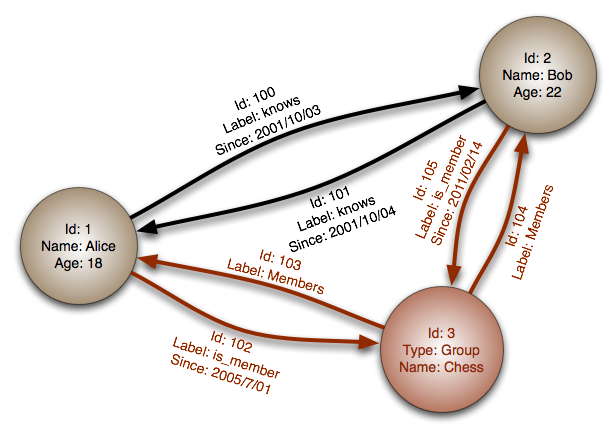
\includegraphics[scale=0.43]{immagini/social.png}
	\caption{\textit{Base di dati per un social network \link{https://goo.gl/Fik4Xp}}}
\end{figure}
\newpage
Un esempio classico di ottimo caso d'uso è quello descritto dalla \hyperlink{fig:social}{figura 3.8}, ossia la modellazione della base di dati di un social network. In questo caso il numero dei nodi, cioè le persone fisiche, sono in numero nettamente minore rispetto alla somma di tutti gli archi, cioè le conoscenze. Inoltre le operazioni che si eseguono coinvolgono sempre una base di dati circoscritta.\\

\subsection{Vantaggi e svantaggi di una base di dato a grafo}
Durante la mia analisi ho riscontrato i seguenti vantaggi e svantaggi nell'utilizzare una base di dati a grafo.
\subsubsection{Vantaggi}
\begin{itemize}
\item{\textbf{Velocità:}} se il caso d'uso è adatto e si organizza i dati in modo intelligente si riesce a ridurre la maggior parte delle \textit{query} ad operazioni banali, sfruttando la natura dei grafi. Nell'ambito anti frode molte operazioni si riducono al "\textit{conta quante volte la persona \textbf{A} ha fatto una determinata cosa, chiamata \textbf{Z}, verso un entità \textbf{B}}" dove A e B sono nodi e Z è l'arco che li collega.
\item{\textbf{Espressività della ricerca:}} se il caso d'uso che si va a modellare è adatto alla natura dei grafi, l'espressività della ricerca è tale che le \textit{query} risultano, molte volte, banali anche dal punto di vista della scrittura.
\item{\textbf{Tutto è collegato:}} data dalla natura dei grafi, si ha un enorme possibilità di creare ricerche che esplorano in profondità il grafo date determinate condizioni, ad esempio la possibilità di attraversare e memorizzare solo i nodi che sono collegati da una determinata entità solamente tramite relazioni di appartenenza. Nell'ambito anti frode succede molto spesso di eseguire delle ricerche che sfruttano questa caratteristica.
\end{itemize}
\subsubsection{Svantaggi}
\begin{itemize}
\item{\textbf{Casi d'uso limitati:}} solo pochi \textit{use case} sono adatti ad essere modellati come un grafo, quindi è molto rischioso modellare totalmente la propria base di dati utilizzando questa tecnologia. Questo perché in futuro potrebbe esserci la necessità di aggiungere dati al modello non adatti a questo tipo di \textit{database}. Questo limita il normale ciclo di vita di un \textit{software}.
\item{\textbf{Tecnologia di nicchia:}} essendo una tecnologia di nicchia la possibilità di informarsi, tramite community, è ridotta rispetto ad altre tecnologie più diffuse, come possono essere i \textit{database} relazionali.
\end{itemize}
\newpage
\begin{figure}[!ht]
	\centering
	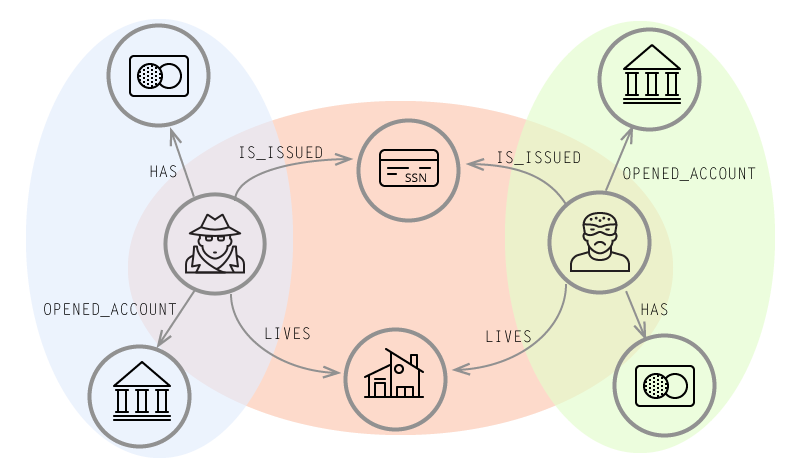
\includegraphics[scale=0.33]{immagini/fraud.png}
	\caption{\textit{Esempio di un caso d'uso orientato all'anti frode \link{http://archive.is/LpXtZ}}}
\end{figure}


\subsection{PRO e CONTRO Neo4j rispetto OrientDB}
\subsubsection{PRO}
\begin{itemize}
\item{\textbf{Espressività:}} chyper, il linguaggio di interrogazione di Neo4j, inizialmente può spaventare, essendo diverso da quelli che siamo abituati a vedere. Dopo un breve periodo di apprendimento risulta, però, facile da utilizzare e molto potente nelle ricerche. Questo è dato dalla sintassi molto regolare ed espressiva con pochissime nozioni.
\item{\textbf{Spring Data Neo4j:}} libreria ben fatta e documentata per astrarre l'interazione con la base di dati, al contrario di OrientDB.
\item{\textbf{Importatore da CSV:}} popolamento della base di dati tramite documento CSV nettamente più veloce rispetto ad OrientDB.
\end{itemize}
\subsubsection{CONTRO}
\begin{itemize}
\item{\textbf{Input/Output lento:}} le librerie di Neo4j, quali Spring Data ed in generale i \textit{driver} java, risultano più lenti rispetto ad quelli di OrientDB. Questo l'ho notato calcolando la differenza tra la velocità netta delle \textit{query}, eseguendola nella \textit{dashboard}, con quella tramite i \textit{driver} e successivamente confrontandola con OrientDB.
\end{itemize}
\subsection{PRO e CONTRO OrientDB rispetto Neo4j}
\subsubsection{PRO}
\begin{itemize}
\item{\textbf{Velocità:}} pur essendo un \textit{database} multi modello la velocità nelle ricerche è comparabile ad una base di dati a grafo.
\end{itemize}
\subsubsection{CONTRO}
\begin{itemize}
\item{\textbf{Spring Data OrientDB:}} non documentato ed acerbo. Questo mi ha portato ad usare Tinkerpop\footnote{Tinkerpop: url= \link{http://tinkerpop.apache.org/}} portando allo sviluppo di un software meno organizzato rispetto a quello di Neo4j.
\item{\textbf{Espressività:}} l'azienda produttrice di OrientDB ha fatto la scelta, per me puramente commerciale, di utilizzare un linguaggio simile ad \gls{SQL} per l'interrogazione della base di dati. Questo diminuisce sostanzialmente l'espressività delle \textit{query}, rendendo complicato lo sviluppo di operazioni con svariate transazioni su archi.
\item{\textbf{Spazio su disco:}} per rendere un database multi modello nativo gli sviluppatori di OrientDB hanno dovuto replicare molti dati, aumentando di circa 0.4 volte lo spazio necessario per immagazzinare i dati (prova eseguita con 30 milioni di record tra nodi ed archi).
\end{itemize}

\subsection{Conclusioni}
Nella parte finale del progetto di stage mi sono posto le seguenti domande per cercare di effettuare una presentazione esaustiva, in azienda, dell'analisi effettuata.\\
\\
\textbf{Vale la pena adottare la base di dati a grafo in azienda?}\\
\textit{Secondo la mia analisi si, però solamente per alcuni casi d'uso.}\\
Adottare un \textit{database} a grafo, e modellare i dati di conseguenza, per determinati casi d'uso renderebbero possibili determinate ricerche che prima potevano risultare troppo onerose o, addirittura, impossibili.\\
Il tratto caratteristico dei \textit{database} a grafo è la possibilità di attraversare, a costo costante, le varie entità ricostruendo le azioni compiute da una particolare entità indipendentemente dalla grandezza della base di dati. Questo aprirebbe, per l'azienda, nuove possibili ricerche come la costruzione dell'albero delle transazioni, dato un utente, per estrapolare determinate informazioni.\\
\\
\textbf{Risolve il problema iniziale del calcolo della reputazione descritto nella \hyperlink{sec:prob}{sezione 2.1.1}?}\\
\textit{Si, almeno utilizzando la base di dati generata casualmente.}\\
Ho eseguito le operazioni in basi di dati con varie unità di grandezze, fino ad arrivare a 30 milioni di transazioni, e il tempo necessario per calcolare la reputazione si aggirava tra i 2 millisecondi per quella totale e i 15 millisecondi per quella relativa. Questo grazie alla possibilità di eseguire queste determinate operazioni senza caricare tutto il \textit{database} in memoria.\\
\\
\\
\textbf{Quale tecnologia utilizzare tra Neo4j e OrientDB?}\\
\textit{Secondo la mia analisi Neo4j.}\\
Ho preso questa decisione analizzandoli nei seguenti 3 ambiti, in ordine di importanza:
\begin{itemize}
\item{\textbf{Espressività:}} il linguaggio di interrogazione di Neo4j è nettamente migliore in termini di espressività. SQL è chiaramente un linguaggio non adatto per le ricerche nei grafi. Al contrario, quello di Neo4j, è sempre espressivo sia in termini di lettura di una \textit{query} sia nel crearla. Questo rende meno costoso, in termini di studio, il cambio tecnologico in azienda. 
\item{\textbf{Supporto alle tecnologie usate in azienda:}} il passaggio a Neo4j risulterebbe meno costoso, in termini di studio individuale, grazie al supporto nativo verso Spring Data. Il supporto di OrientDB verso questa tecnologia risulta ancora acerba.

\item{\textbf{Velocità:}} in termini di velocità di esecuzione di una \textit{query} Neo4j migliore, sopratutto all'aumentare delle transazioni sui nodi.
\end{itemize}
















% !TEX encoding = UTF-8
% !TEX TS-program = pdflatex
% !TEX root = ../tesi.tex

%**************************************************************
\chapter{Valutazione}
\label{cap:resoconto-stage}
%**************************************************************

%**************************************************************
\section{Soddisfacimento degli obiettivi}
Il progetto di stage ha avuto una durata di 316 ore, oltre la durata minima ma in linea con quella massima di 320 ore.\\
Negli ultimi due giorni di stage ho preparato, e successivamente esposto, una presentazione del lavoro svolto, durante il periodo di stage, al mio tutor, Giuseppe Pavan, al \textit{team leader} e sviluppatore \textit{senior}, Riccardo Cardin, e al CTO di \textit{\azienda}, Guido Ronchetti \footnote{Guido Ronchetti: Linkedin= \link{https://www.linkedin.com/in/guido-ronchetti-285637a/}}. Grazie a questa presentazione ho potuto ricevere un \textit{feedback} del lavoro svolto, riassumere al \textit{team} dell'azienda che mi ha ospitato la mia analisi tecnologica e le idee su questi tipi di base di dati ed, infine, fare esperienza nella preparazione di un discorso tecnico da esporre a persone con esperienza decennale.\\
Attraverso i documenti consegnati, il prototipo e la presentazione da me svolti, l'azienda ha potuto acquisire le informazioni necessarie per valutare il passaggio a questo tipo di tecnologia. Chiaramente questo mio progetto non può sostituire una vera analisi di fattibilità con i relativi costi per lo studio di nuove tecnologie e conseguenze tecniche dovute al cambiamento. Il mio prodotto potrà servire, però, all'azienda per determinare se vale la pena svolgere questo tipo di attività e individuare nuove funzionalità dovute al cambiamento. Tutto questo risparmiando sia risorse sia tempo, che a volte in un azienda possono essere limitate.\\
Gli obiettivi obbligatori, come descritto nella \hyperlink{sec:pianodl}{sezione 2.1.3}, si concentravano sull'analisi delle varie tecnologie di basi di dati a grafo e sulla progettazione e realizzazione di un prototipo che esemplifichi le capacità di queste. Sono stati soddisfatti completamente risparmiando un numero significativo di ore lavoro. Con le ore rimaste mi sono concentrato nel migliorare il prototipo, aggiungendo funzionalità interessanti, e nel soddisfare un requisito opzionale, cioè la preparazione di una presentazione interna del lavoro svolto.
\newpage
\section{Conoscenze acquisite}
Le conoscenze che, grazie a questa esperienza di stage, ho acquisito o semplicemente ampliato sono le seguenti.
\subsubsection{Base di dati a grafo}
Durante questo progetto ho potuto avvicinarmi ai \textit{database} organizzati a grafo, tecnologia che ignoravo prima di questa esperienza.\\
Inizialmente, questa tecnologia mi è sembrata simile alle basi di dati relazionali. Informandomi e testandola con il mio prototipo, però, ho compreso le sue potenzialità. Quasi tutti i vantaggi sono dati dalla possibilità di attraversare i nodi in tempo costante e non dipendente dalla grandezza del \textit{database}, questo non avviene in quelli relazionali a causa delle operazioni di \gls{JOIN}.\\
Mi ritengo soddisfatto di aver acquisito delle conoscenze in questa materia grazie all'evoluzione che sta avendo in questo ultimo periodo, rispetto alle altre tipologie di base di dati.
\begin{figure}[h!]
	\centering
	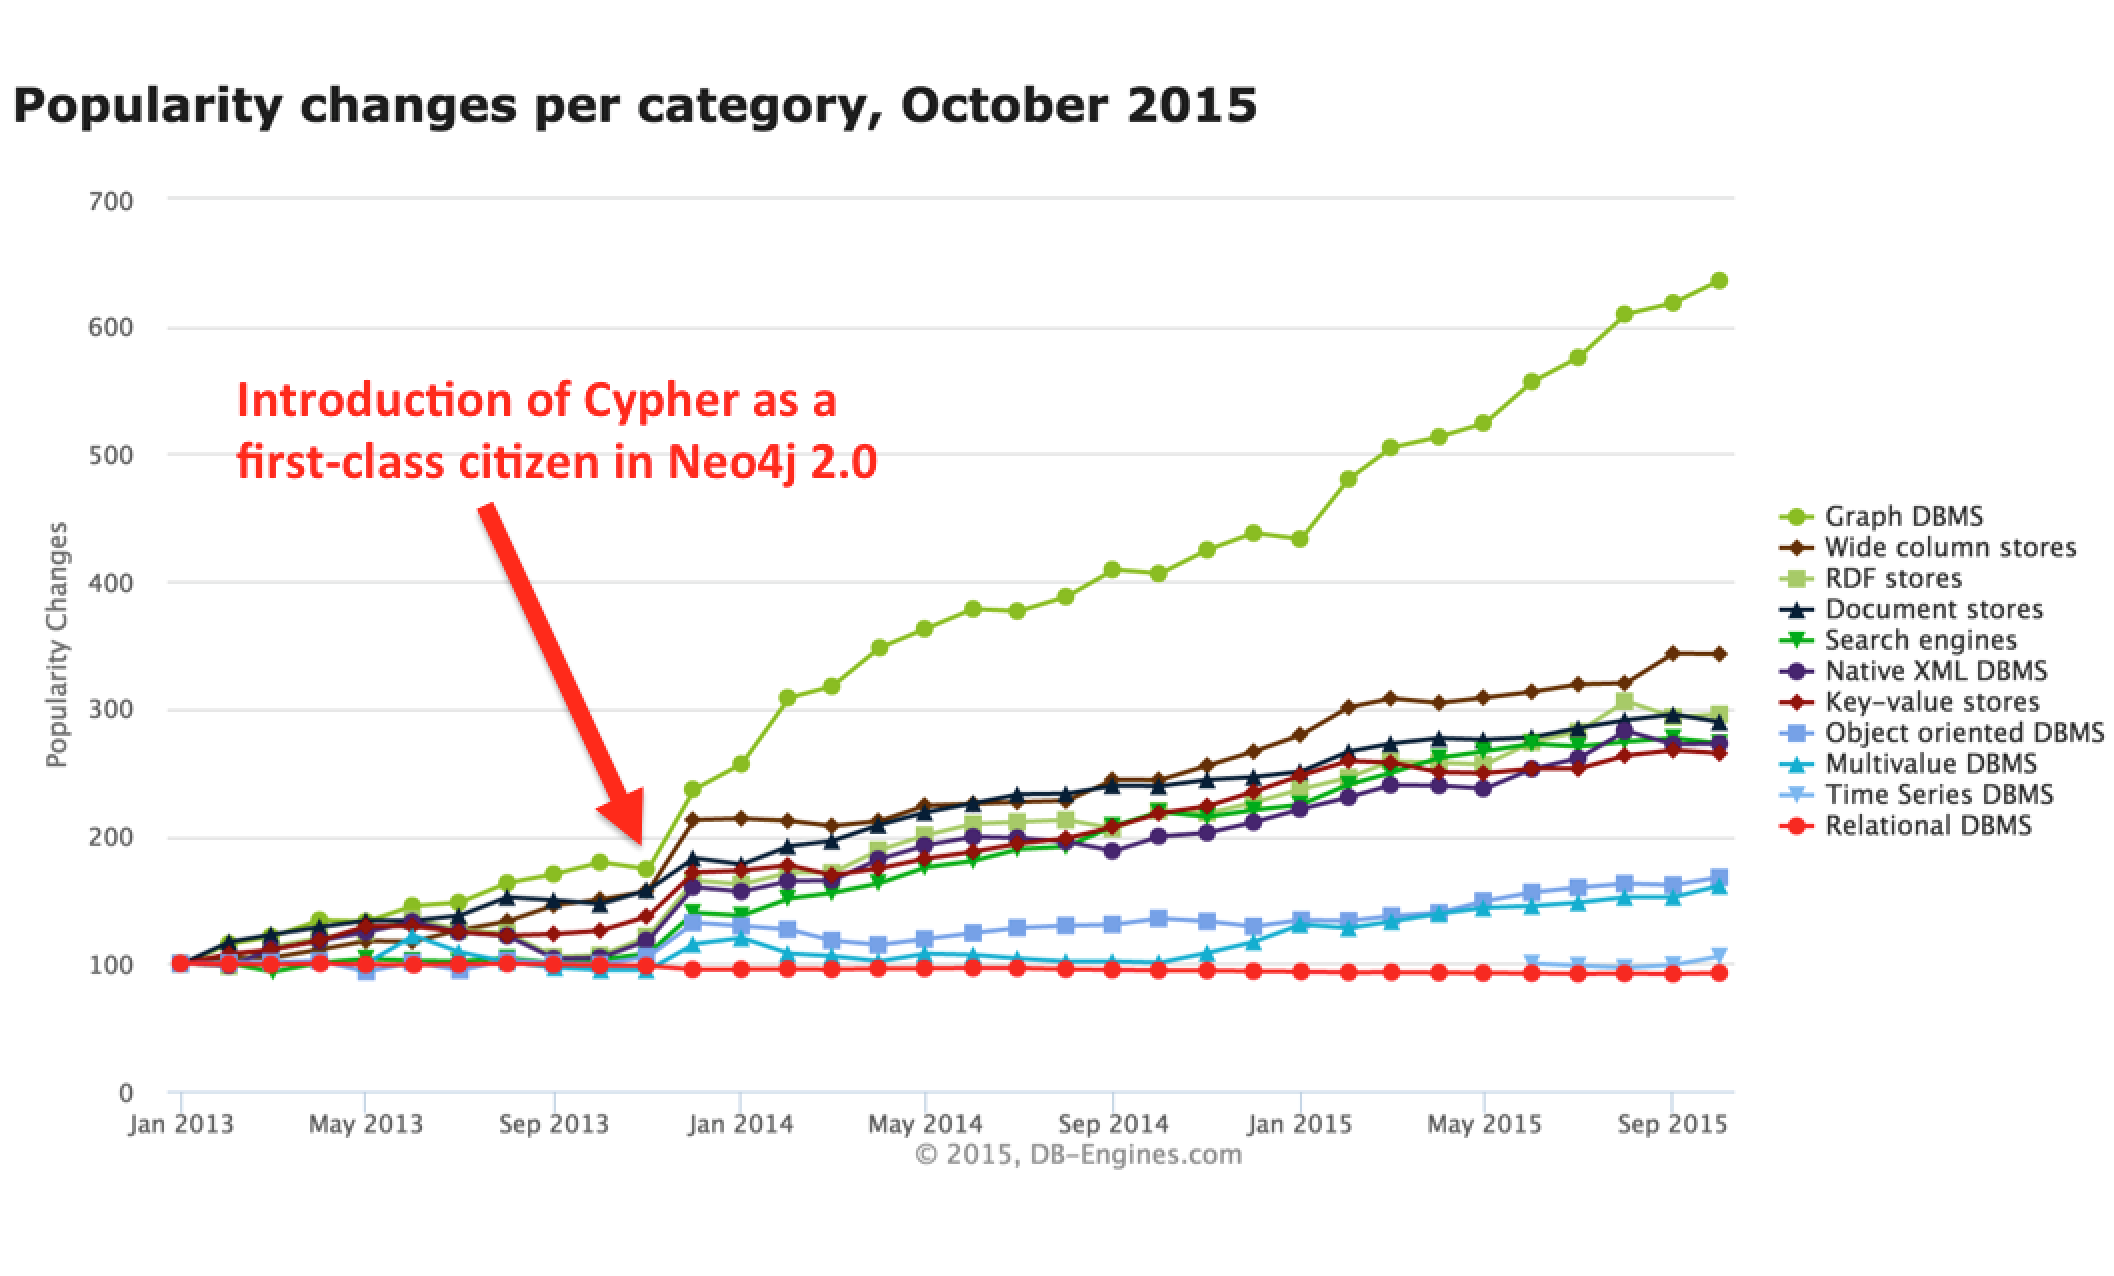
\includegraphics[scale=0.4]{immagini/graphchange.png}
	\label{fig:figura 2.2}
	\caption{\textit{Evoluzioni delle base di dati a grafo rispetto alle altre tipologie \link{https://goo.gl/SfV3vZ}}}
\end{figure}
\newpage
\subsubsection{Capacità di condurre una analisi tecnologica}
Attraverso questa esperienza ho potuto acquisire capacità di condurre una analisi tecnologica strutturata. Ho imparato ad individuare le possibili alternative, eseguire una scrematura utilizzando un confronto strutturato ed uniforme per caratteristiche ed, infine, scegliere la migliore in base al caso d'uso di riferimento. Tutto questo aiutandomi con le documentazioni ufficiali delle alternative tecnologiche e \textit{forum} di riferimento quali StackOverflow\footnote{StackOverflow: url= \link{https://stackoverflow.com/}} e Dzone\footnote{Dzone: url= \link{https://dzone.com/}}.
\subsubsection{Progettazione e realizzazione di un'applicazione Java}
Ho potuto acquisire capacità di progettare e realizzare autonomamente una applicazione Java sfruttando \textit{\gls{framework}} avanzati come Spring\footnote{Spring: url= \link{https://spring.io/}} e utilizzare, anche se superficialmente, la tecnologia Docker\footnote{Docker: url= \link{https://www.docker.com/}}.
\section{Valutazione personale}
Per quanto riguarda questa esperienza di stage mi ritengo soddisfatto del lavoro svolto, in termini di requisiti e qualità del prodotto finale, e del progetto di stage scelto. Purtroppo non ho potuto soddisfare completamente i requisiti opzionali sia per mancanza di tempo che per l'impossibilità di recuperare, o solamente analizzare, dati reali per le stringenti politiche sulla \textit{privacy} di dati sensibili.\\
Mi ritengo soddisfatto, invece, del progetto scelto perchè lo ritengo un giusto compromesso tra una analisi, che mi ha portato a svolgere una tesi con buoni contenuti, ed un progetto di sviluppo che mi ha permesso di acquisire conoscenze che sfrutterò nel mondo del lavoro.\\
Infine ritengo il progetto di stage, in un azienda esterna, l'unico modo per acquisire nozioni che durante il corso di studi sarebbe molto difficile conseguire in così poco tempo. Personalmente estenderei l'obbligo di stage a molti altri corsi di studi universitari che non lo contengono.
\section{Differenza tra università e mondo del lavoro}
Durante la mia esperienza lavorativa ho notato un \textit{gap} rispetto al percorso di studi universitario. Questa differenza si focalizza nella mancanza di conoscenza nelle tecnologie avanzate, come particolari \textit{\gls{framework}}, oppure di nuova generazione. Questa mancanza è sopperita, però, dall'insegnamento durante i corsi universitari dei concetti di base che mi hanno portato ad imparare ed adattarmi velocemente a queste nuove tecnologie. Ciò non significa che non si debba aggiorare i percorsi di studi con un programma adatto al mondo lavorativo odierno.\\ Personalmente valuterei l'aggiunta, da parte dell'università, di un insegnamento che avvicini lo studente alle basi di dati non relazionali e l'uso avanzato di Java, spiegando le nuove funzionalità introdotte con le recenti versioni di questo linguaggio.\\
Inoltre aggiungerei, ad un corso già presente, un avvicinamento ai sistemi di controllo di versione, invece di delegare totalmente allo studente l'onere di impararlo durante gli svariati progetti universitari.\\
Un'altra cosa che mi ha lasciato perplesso durante il mio percorso universitario è stata la scelta di non insegnare, nel corso di tecnologie \textit{web}, tecnologie di rilievo, anche se non definite da \textit{standard}, come HTML5\footnote{HTML5: url= \link{https://www.w3schools.com/html/html5\textunderscore intro.asp}}.\\
Al netto di questi dettagli il mio percorso di studi mi ha permesso di acquisire nozioni ed aspetti fondamentali dell'informatica che non sarei riuscito ad imparare autonomamente. Inoltre è riuscito a far si che mi appassionassi alla materia nonostante, prima dell'iscrizione all'Università di Padova, la mia conoscenza a questa fosse nulla. \\Considero molto importante la presenza dei progetti universitari: mi hanno insegnato a lavorare in un \textit{team}, mantenuto alta la voglia di migliorarmi e permesso di aggiungere un'esperienza dimostrabile al mio \textit{curriculum}, oltre a tutte le nozioni tecniche che ho appreso.


%\appendix                               
%\input{capitoli/capitolo-A}             % Appendice A

%**************************************************************
% Materiale finale
%**************************************************************
%\backmatter
%\printglossaries
%% !TEX encoding = UTF-8
% !TEX TS-program = pdflatex
% !TEX root = ../tesi.tex

%**************************************************************
% Bibliografia
%**************************************************************

\cleardoublepage
\chapter{Bibliografia}

\section{Siti Consultati}
\textit{Neo4j:} \link{https://neo4j.com/}\\
\\
\textit{OrienDB:} \link{http://orientdb.com/orientdb/}\\
\\
\textit{ArangoDB:} \link{https://www.arangodb.com/}\\
\\
\textit{AllegroGraph:} \link{https://franz.com/agraph/allegrograph/}\\
\\
\textit{TitanDB:} \link{http://titan.thinkaurelius.com/}\\
\\
\textit{DZone:} \link{https://dzone.com/}\\
\\
\textit{StackOverlow:} \link{https://stackoverflow.com/}\\
\\
\textit{Spring:} \link{https://spring.io/}\\
\\
\textit{Docker:} \link{https://www.docker.com/}\\
\\
\textit{Apache Tinkerpop:} \link{http://tinkerpop.apache.org/}\\



\end{document}